\mfpicnumber{1}

\opengraphsfile{Transformations}

\setcounter{footnote}{0}

\label{Transformations}

In this section, we study how the graphs of functions change, or \textbf{transform}, when certain specialized modifications are made to their formulas. The transformations we will study fall into three broad categories:  shifts, reflections and scalings, and we will present them in that order.  Suppose the graph below is the complete graph of a function $f$.\index{transformations of function graphs}\index{function ! transformation of graphs}

\begin{center}

\begin{mfpic}[15]{-1}{6}{-1}{6}
\polyline{(0,1), (2,3), (4,3), (5,5)}
\point[3pt]{(0,1), (2,3), (4,3), (5,5)}
\tlabel[cc](-1,1){\scriptsize $(0,1)$}
\tlabel[cc](2,3.5){\scriptsize $(2,3)$}
\tlabel[cc](4,2.5){\scriptsize $(4,3)$}
\tlabel[cc](5,5.5){\scriptsize $(5,5)$}
\tlabel[cc](6,-0.5){\scriptsize $x$}
\tlabel[cc](0.5,6){\scriptsize $y$}
\tcaption{\scriptsize $y=f(x)$}
\axes
\xmarks{1,2,3,4,5}
\ymarks{1,2,3,4,5}
\tlpointsep{4pt}
\axislabels {x}{{\tiny $1$} 1, {\tiny $2$} 2, {\tiny $3$} 3, {\tiny $4$} 4, {\tiny $5$} 5}
\axislabels {y}{{\tiny $2$} 2, {\tiny $3$} 3, {\tiny $4$} 4, {\tiny $5$} 5}
\end{mfpic}

\end{center}

The Fundamental Graphing Principle for Functions says that for a point $(a,b)$ to be on the graph, $f(a) = b$.  In particular, we know $f(0) = 1$, $f(2)=3$, $f(4)=3$ and $f(5)=5$.  Suppose we wanted to graph the function defined by the formula $g(x) = f(x) + 2$.  Let's take a minute to remind ourselves of what $g$ is doing.  We start with an input $x$ to the function $f$ and we obtain the output $f(x)$.  The function $g$ takes the output $f(x)$ and adds $2$ to it.  In order to graph $g$, we need to graph the points $(x,g(x))$.  How are we to find the values for $g(x)$ without a formula for $f(x)$?  The answer is that we don't need a \textit{formula} for $f(x)$, we just need the \textit{values} of $f(x)$.  The values of $f(x)$ are the $y$ values on the graph of $y=f(x)$.  For example, using the points indicated on the graph of $f$, we can make the following table.

\[ \begin{array}{|c||c|c|c|c|}  

\hline

 x & (x,f(x)) & f(x) & g(x)=f(x)+2 & (x, g(x)) \\ \hline
0  & (0,1)& 1 & 3 &(0, 3) \\  \hline
2 & (2,3) & 3 &  5 &(2,5) \\  \hline
4 & (4,3) & 3 &  5 &(4, 5) \\  \hline
5 & (5,5) & 5 &  7 &( 5 ,7) \\  \hline

\end{array} \] 

In general, if $(a,b)$ is on the graph of $y=f(x)$, then $f(a) = b$, so $g(a) = f(a) +2 = b+2$.  Hence, $(a,b+2)$ is on the graph of $g$. In other words, to obtain the graph of $g$, we add $2$ to the $y$-coordinate of each point on the graph of $f$.  Geometrically, adding $2$ to the $y$-coordinate of a point moves the point $2$ units above its previous location.  Adding $2$ to every $y$-coordinate on a graph \textit{en masse} is usually described as `shifting the graph up $2$ units'.  Notice that the graph retains the same basic shape as before, it is just $2$ units above its original location.  In other words, we connect the four points we moved in the same manner in which they were connected before.  We have the results side-by-side at the top of the next page.

\[ \begin{array}{ccc}

\begin{mfpic}[15]{-1}{6}{-1}{8}
\polyline{(0,1), (2,3), (4,3), (5,5)}
\point[3pt]{(0,1), (2,3), (4,3), (5,5)}
\tlabel[cc](-1,1){\scriptsize $(0,1)$}
\tlabel[cc](2,3.5){\scriptsize $(2,3)$}
\tlabel[cc](4,2.5){\scriptsize $(4,3)$}
\tlabel[cc](5,5.5){\scriptsize $(5,5)$}
\tlabel[cc](6,-0.5){\scriptsize $x$}
\tlabel[cc](0.5,8){\scriptsize $y$}
\tcaption{\scriptsize $y=f(x)$}
\axes
\xmarks{1,2,3,4,5}
\ymarks{1,2,3,4,5,6,7}
\tlpointsep{4pt}
\axislabels {x}{{\tiny $1$} 1, {\tiny $2$} 2, {\tiny $3$} 3, {\tiny $4$} 4, {\tiny $5$} 5}
\axislabels {y}{{\tiny $2$} 2,  {\tiny $3$} 3, {\tiny $4$} 4, {\tiny $5$} 5, {\tiny $6$} 6, {\tiny $7$} 7}
\end{mfpic}

&

\stackrel{\stackrel{\mbox{\scriptsize shift up $2$ units}}{\xrightarrow{\hspace{1in}}}}{\mbox{ \scriptsize add $2$ to each $y$-coordinate}} 

& 

\begin{mfpic}[15]{-1}{6}{-1}{8}
\polyline{(0,3), (2,5), (4,5), (5,7)}
\point[3pt]{(0,3), (2,5), (4,5), (5,7)}
\tlabel[cc](-1,3){\scriptsize $(0,3)$}
\tlabel[cc](2,5.5){\scriptsize $(2,5)$}
\tlabel[cc](4,4.5){\scriptsize $(4,5)$}
\tlabel[cc](5,7.5){\scriptsize $(5,7)$}
\tlabel[cc](6,-0.5){\scriptsize $x$}
\tlabel[cc](0.5,8){\scriptsize $y$}
\tcaption{\scriptsize $y=g(x) = f(x)+2$}
\axes
\xmarks{1,2,3,4,5}
\ymarks{1,2,3,4,5,6,7}
\tlpointsep{4pt}
\axislabels {x}{{\tiny $1$} 1, {\tiny $2$} 2, {\tiny $3$} 3, {\tiny $4$} 4, {\tiny $5$} 5}
\axislabels {y}{{\tiny $1$} 1,{\tiny $2$} 2,  {\tiny $4$} 4, {\tiny $5$} 5, {\tiny $6$} 6, {\tiny $7$} 7}
\end{mfpic} \end{array}\]
 
You'll note that the domain of $f$ and the domain of $g$ are the same, namely $[0,5]$, but that the range of $f$ is $[1,5]$ while the range of $g$ is $[3,7]$.  In general, shifting a function vertically like this will leave the domain unchanged, but could very well affect the range.  You can easily imagine what would happen if we wanted to graph the function $j(x) = f(x) - 2$.  Instead of adding $2$ to each of the $y$-coordinates on the graph of $f$, we'd be subtracting $2$.  Geometrically, we would be moving the graph down $2$ units.  We leave it to the reader to verify that the domain of $j$ is the same as $f$, but the range of $j$ is $[-1,3]$.  What we have discussed is generalized in the following theorem.

\smallskip

\colorbox{ResultColor}{\bbm

%\smallskip

\begin{thm} \label{vshifts}\textbf{Vertical Shifts.}\index{graph ! vertical shift} Suppose $f$ is a function and $k$ is a positive number. 

\begin{itemize}

\item To graph $y=f(x)+k$, shift the graph of $y=f(x)$ up $k$ units by adding $k$ to the $y$-coordinates of the points on the graph of $f$.

\item To graph $y=f(x)-k$, shift the graph of $y=f(x)$ down $k$ units by subtracting $k$ from the $y$-coordinates of the points on the graph of $f$.

\end{itemize}

\end{thm}

\ebm}

\smallskip

The key to understanding Theorem \ref{vshifts} and, indeed, all of the theorems in this section comes from an  understanding of the Fundamental Graphing Principle for Functions.  If $(a,b)$ is on the graph of $f$, then $f(a) = b$.  Substituting $x=a$ into the equation  $y=f(x)+k$ gives $y=f(a)+k = b+k$.  Hence, $(a,b+k)$ is on the graph of $y=f(x)+k$, and we have the result.  In the language of `inputs' and `outputs', Theorem \ref{vshifts} can be paraphrased as ``Adding to, or subtracting from, the \textit{output} of a function causes the graph to shift up or down, respectively.''   So what happens if we add to or subtract from the \textit{input} of the function?  

\smallskip

Keeping with the graph of $y=f(x)$ above, suppose we wanted to graph $g(x) = f(x+2)$.  In other words, we are looking to see what happens when we add $2$ to the input of the function.\footnote{We have spent a lot of time in this text showing you that $f(x+2)$ and $f(x)+2$ are, in general, wildly different algebraic animals.   We will see momentarily that their geometry is also dramatically different.}  Let's try to generate a table of values of $g$ based on those we know for $f$.  We quickly find that we run into some difficulties.

\[ \begin{array}{|c||c|c|c|c|}  

\hline

x & (x,f(x)) & f(x)& g(x)=f(x+2) & (x, g(x)) \\ \hline
0  & (0,1)& 1 & f(0+2) = f(2) = 3   &(0, 3) \\  \hline
2 & (2,3) & 3 & f(2+2) = f(4) = 3  &(2,3) \\  \hline
4 & (4,3) & 3 &  f(4+2) = f(6) = ? &  \\  \hline
5 & (5,5) & 5 & f(5+2) = f(7) = ?  &  \\  \hline

\end{array} \] 

When we substitute $x=4$ into the formula $g(x)=f(x+2)$, we are asked to find $f(4+2)=f(6)$ which doesn't exist because the domain of $f$ is only $[0,5]$.  The same thing happens when we attempt to find $g(5)$.  What we need here is a new strategy.  We know, for instance, $f(0) = 1$.  To determine the corresponding point on the graph of $g$, we need to figure out what value of $x$ we must substitute into $g(x) = f(x+2)$ so that the quantity $x+2$, works out to be $0$.  Solving $x+2=0$ gives $x=-2$, and $g(-2) = f((-2)+2) = f(0) = 1$ so  $(-2,1)$ on the graph of $g$.  To use the fact $f(2) = 3$, we set $x+2 = 2$ to get $x=0$. Substituting gives $g(0) = f(0+2) = f(2) = 3$.  Continuing in this fashion, we get  \[ \begin{array}{|r||c|c|c|}  

\hline

x & x+2 & g(x)=f(x+2) & (x, g(x)) \\ \hline
-2 & 0 & g(-2)=f(0) = 1   &(-2, 1) \\  \hline
0 &  2 &  g(0)=f(2) = 3  &(0,3) \\  \hline
2 & 4  & g(2)=f(4) = 3 &  (2,3)\\  \hline
3 & 5 & g(3)=f(5) = 5  & (3,5) \\  \hline

\end{array} \] 

In summary, the points $(0,1)$, $(2,3)$, $(4,3)$ and $(5,5)$ on the graph of $y=f(x)$ give rise to the points  $(-2,1)$, $(0,3)$, $(2,3)$ and $(3,5)$ on the graph of $y=g(x)$, respectively.  In general, if $(a,b)$ is on the graph of $y=f(x)$, then $f(a) = b$.  Solving $x+2 = a$ gives $x = a-2$ so that $g(a-2) = f((a-2)+2) = f(a) = b$.  As such, $(a-2,b)$ is on the graph of $y=g(x)$. The point $(a-2,b)$ is exactly $2$ units to the \emph{left} of the point $(a,b)$ so the graph of $y=g(x)$ is obtained by shifting the graph $y=f(x)$ to the left $2$ units, as pictured below.

\[\begin{array}{ccc}

\begin{mfpic}[15]{-3}{6}{-1}{6}
\polyline{(0,1), (2,3), (4,3), (5,5)}
\point[3pt]{(0,1), (2,3), (4,3), (5,5)}
\tlabel[cc](-1,1){\scriptsize $(0,1)$}
\tlabel[cc](2,3.5){\scriptsize $(2,3)$}
\tlabel[cc](4,2.5){\scriptsize $(4,3)$}
\tlabel[cc](5,5.5){\scriptsize $(5,5)$}
\tlabel[cc](6,-0.5){\scriptsize $x$}
\tlabel[cc](0.5,6){\scriptsize $y$}
\tcaption{\scriptsize $y=f(x)$}
\axes
\xmarks{-2,-1, 1,2,3,4,5}
\ymarks{1,2,3,4,5}
\tlpointsep{4pt}
\axislabels {x}{{\tiny $-2 \hspace{7pt}$} -2, {\tiny $-1\hspace{7pt}$} -1,{\tiny $1$} 1, {\tiny $2$} 2, {\tiny $3$} 3, {\tiny $4$} 4, {\tiny $5$} 5}
\axislabels {y}{{\tiny $2$} 2, {\tiny $3$} 3, {\tiny $4$} 4, {\tiny $5$} 5}
\end{mfpic} 

&

\stackrel{\stackrel{\mbox{\scriptsize shift left $2$ units}}{\xrightarrow{\hspace{1in}}}}{\mbox{ \scriptsize subtract $2$ from each $x$-coordinate}} 

& 

\begin{mfpic}[15]{-3}{6}{-1}{6}
\polyline{(-2,1), (0,3), (2,3), (3,5)}
\point[3pt]{(-2,1), (0,3), (2,3), (3,5)}
\tlabel[cc](-3,1){\scriptsize $(-2,1)$}
\tlabel[cc](-1,3){\scriptsize $(0,3)$}
\tlabel[cc](2,2.5){\scriptsize $(2,3)$}
\tlabel[cc](3,5.5){\scriptsize $(3,5)$}
\tlabel[cc](6,-0.5){\scriptsize $x$}
\tlabel[cc](0.5,6){\scriptsize $y$}
\tcaption{\scriptsize $y=g(x)=f(x+2)$}
\axes
\xmarks{-2,-1, 1,2,3,4,5}
\ymarks{1,2,3,4,5}
\tlpointsep{4pt}
\axislabels {x}{{\tiny $-2 \hspace{7pt}$} -2, {\tiny $-1\hspace{7pt}$} -1,{\tiny $1$} 1, {\tiny $2$} 2, {\tiny $3$} 3, {\tiny $4$} 4, {\tiny $5$} 5}
\axislabels {y}{{\tiny $1$} 1, {\tiny $2$} 2, {\tiny $4$} 4, {\tiny $5$} 5}
\end{mfpic}

\end{array}\]

Note that while the ranges of $f$ and $g$ are the same, the domain of $g$ is $[-2,3]$ whereas the domain of $f$ is $[0,5]$.  In general, when we shift the graph horizontally, the range will remain the same, but the domain could change.  If we set out to graph $j(x) = f(x-2)$, we would find ourselves \textit{adding} $2$ to all of the $x$ values of the points on the graph of $y=f(x)$ to effect a shift to the \emph{right} $2$ units. Generalizing these notions produces the following result.

\smallskip

\colorbox{ResultColor}{\bbm

%\smallskip

\begin{thm} \label{hshifts}\textbf{Horizontal Shifts.}\index{graph ! horizontal shift}  Suppose $f$ is a function and $h$ is a positive number. 

\begin{itemize}

\item To graph $y=f(x+h)$, shift the graph of $y=f(x)$ left $h$ units by subtracting $h$ from the $x$-coordinates of the points on the graph of $f$.

\item To graph $y=f(x-h)$, shift the graph of $y=f(x)$ right $h$ units by adding $h$ to the $x$-coordinates of the points on the graph of $f$.

\end{itemize}

\end{thm}

\ebm}

\smallskip

In other words,  Theorem \ref{hshifts} says that adding to or subtracting from the  \textit{input} to a function amounts to shifting the graph left or right, respectively.  Theorems \ref{vshifts} and \ref{hshifts} present a theme which will run common throughout the section:  changes to the outputs from a function affect the $y$-coordinates of the graph, resulting in some kind of vertical change;  changes to the inputs to a function affect the $x$-coordinates of the graph, resulting in some kind of horizontal change.

\begin{ex}  $~$ \label{transformationex1}

\begin{enumerate}

\item  Graph $f(x) = \sqrt{x}$.  Plot at least three points. 

\item  Use your graph in 1 to graph $g(x) = \sqrt{x}-1$. 

\item  Use your graph in 1 to graph  $j(x) = \sqrt{x-1}$.

\item  Use your graph in 1 to graph $m(x) = \sqrt{x+3} - 2$. 

\end{enumerate}

\smallskip

{\bf Solution.}  

\begin{enumerate}

\item  Owing to the square root, the domain of $f$ is $x \geq 0$, or $[0,\infty)$.  We choose perfect squares to build our table and graph below.  From the graph we verify the domain of $f$ is $[0,\infty)$ and the range of $f$ is also $[0, \infty)$.

\begin{tabular}{m{0.5in}m{3in}m{3in}}

&

$\begin{array}{|c||c|c|}  

\hline

x & f(x) & (x,f(x)) \\ \hline
0  & 0& (0,0)  \\  \hline
1 & 1 & (1,1)  \\  \hline
4 & 2 & (4,2)  \\  \hline

\end{array}$ & 

\begin{mfpic}[15]{-1}{5}{-1}{3}
\arrow \function{0,5,0.1}{sqrt(x)}
\point[3pt]{(0,0), (1,1), (4,2)}
\tlabel[cc](-1,0.25){\scriptsize $(0,0)$}
\tlabel[cc](1,1.5){\scriptsize $(1,1)$}
\tlabel[cc](4,2.5){\scriptsize $(4,2)$}
\tlabel[cc](5,-0.5){\scriptsize $x$}
\tlabel[cc](0.5,3){\scriptsize $y$}
\tcaption{\scriptsize $y=f(x)=\sqrt{x}$}
\axes
\xmarks{1,2,3,4}
\ymarks{1,2}
\tlpointsep{4pt}
\axislabels {x}{{\tiny $1$} 1, {\tiny $2$} 2, {\tiny $3$} 3, {\tiny $4$} 4}
\axislabels {y}{{\tiny $1$} 1, {\tiny $2$} 2}
\end{mfpic}

\end{tabular}

\item The domain of $g$ is the same as the domain of $f$, since the only condition on both functions is that $x \geq 0$.  If we compare the formula for $g(x)$ with $f(x)$, we see that $g(x) = f(x) - 1$.  In other words, we have subtracted $1$ from the output of the function $f$. By Theorem \ref{vshifts}, we know that in order to graph $g$, we shift the graph of $f$ down one unit by subtracting $1$ from each of the $y$-coordinates of the points on the graph of $f$.  Applying this to the three points we have specified on the graph, we move $(0,0)$ to $(0,-1)$, $(1,1)$ to $(1,0)$, and $(4,2)$ to $(4,1)$.  The rest of the points follow suit, and we connect them with the same basic shape as before. We confirm the domain of $g$ is $[0, \infty)$ and find the range of $g$ to be $[-1, \infty)$.

\[ \begin{array}{ccc}

\begin{mfpic}[15]{-1}{5}{-2}{3}
\arrow \function{0,5,0.1}{sqrt(x)}
\point[3pt]{(0,0), (1,1), (4,2)}
\tlabel[cc](-1,0.25){\scriptsize $(0,0)$}
\tlabel[cc](1,1.5){\scriptsize $(1,1)$}
\tlabel[cc](4,2.5){\scriptsize $(4,2)$}
\tlabel[cc](5,-0.5){\scriptsize $x$}
\tlabel[cc](0.5,3){\scriptsize $y$}
\tcaption{\scriptsize $y=f(x)=\sqrt{x}$}
\axes
\xmarks{1,2,3,4}
\ymarks{-1,1,2}
\tlpointsep{4pt}
\axislabels {x}{{\tiny $1$} 1, {\tiny $2$} 2, {\tiny $3$} 3, {\tiny $4$} 4}
\axislabels {y}{{\tiny $1$} 1,{\tiny $2$} 2}
\end{mfpic}

&

\stackrel{\stackrel{\mbox{\scriptsize shift down $1$ unit}}{\xrightarrow{\hspace{1in}}}}{\mbox{ \scriptsize subtract $1$ from each $y$-coordinate}} 

&

\begin{mfpic}[15]{-1}{5}{-2}{3}
\arrow \function{0,5,0.1}{sqrt(x)-1}
\point[3pt]{(0,-1), (1,0), (4,1)}
\tlabel[cc](-1,-1){\scriptsize $(0,-1)$}
\tlabel[cc](1,0.5){\scriptsize $(1,0)$}
\tlabel[cc](4,1.5){\scriptsize $(4,1)$}
\tlabel[cc](5,-0.5){\scriptsize $x$}
\tlabel[cc](0.5,3){\scriptsize $y$}
\tcaption{\scriptsize $y=g(x)=\sqrt{x}-1$}
\axes
\xmarks{1,2,3,4}
\ymarks{-1,1,2}
\tlpointsep{4pt}
\axislabels {x}{{\tiny $1$} 1, {\tiny $2$} 2, {\tiny $3$} 3, {\tiny $4$} 4}
\axislabels {y}{{\tiny $1$} 1,{\tiny $2$} 2}
\end{mfpic}

\end{array}\]

\item  Solving $x-1 \geq 0$ gives $x \geq 1$, so the domain of $j$ is $[1,\infty)$.  To graph $j$, we note that $j(x) = f(x-1)$.  In other words, we are subtracting $1$ from the \textit{input} of $f$.  According to Theorem \ref{hshifts}, this induces a shift to the right of the graph of $f$.  We add $1$ to the $x$-coordinates of the points on the graph of $f$ and get the result below.  The graph reaffirms that the domain of $j$ is  $[1,\infty)$ and tells us that the range of $j$ is $[0,\infty)$.

\[ \begin{array}{ccc}

\begin{mfpic}[15]{-1}{6}{-1}{3}
\arrow \function{0,5,0.1}{sqrt(x)}
\point[3pt]{(0,0), (1,1), (4,2)}
\tlabel[cc](-1,0.25){\scriptsize $(0,0)$}
\tlabel[cc](1,1.5){\scriptsize $(1,1)$}
\tlabel[cc](4,2.5){\scriptsize $(4,2)$}
\tlabel[cc](6,-0.5){\scriptsize $x$}
\tlabel[cc](0.5,3){\scriptsize $y$}
\tcaption{\scriptsize $y=f(x)=\sqrt{x}$}
\axes
\xmarks{1,2,3,4}
\ymarks{1,2}
\tlpointsep{4pt}
\axislabels {x}{{\tiny $1$} 1, {\tiny $2$} 2, {\tiny $3$} 3, {\tiny $4$} 4, {\tiny $5$} 5}
\axislabels {y}{{\tiny $1$} 1, {\tiny $2$} 2}
\end{mfpic}

&

\stackrel{\stackrel{\mbox{\scriptsize shift right $1$ unit}}{\xrightarrow{\hspace{1in}}}}{\mbox{ \scriptsize add $1$ to each $x$-coordinate}} 

&

\begin{mfpic}[15]{-1}{6}{-1}{3}
\arrow \function{1,6,0.1}{sqrt(x-1)}
\point[3pt]{(1,0), (2,1), (5,2)}
\tlabel[cc](1,-0.5){\scriptsize $(1,0)$}
\tlabel[cc](2,1.5){\scriptsize $(2,1)$}
\tlabel[cc](5,2.5){\scriptsize $(5,2)$}
\tlabel[cc](6,-0.5){\scriptsize $x$}
\tlabel[cc](0.5,3){\scriptsize $y$}
\tcaption{\scriptsize $y=j(x)=\sqrt{x-1}$}
\axes
\xmarks{1,2,3,4,5}
\ymarks{1,2}
\tlpointsep{4pt}
\axislabels {x}{ {\tiny $2$} 2, {\tiny $3$} 3, {\tiny $4$} 4, {\tiny $5$} 5}
\axislabels {y}{{\tiny $1$} 1, {\tiny $2$} 2}
\end{mfpic}

\end{array}\]

\item  To find the domain of $m$, we solve $x+3 \geq 0$ and get $[-3, \infty)$.  Comparing the formulas of $f(x)$ and $m(x)$, we have $m(x) = f(x+3) - 2$.  We have $3$ being added to an input, indicating a horizontal shift,  and $2$ being subtracted from an output, indicating a vertical shift. We leave it to the reader to verify that, in this particular case, the order in which we perform these transformations is immaterial;  we will arrive at the same graph regardless as to which transformation we apply first.\footnote{We shall see in the next example that order is  generally important when applying more than one transformation to a graph.} We follow the convention `inputs first',\footnote{We could equally have chosen the convention `outputs first'.} and to that end we first tackle the horizontal shift.  Letting $m_{\mbox{\tiny$1$}}(x) = f(x+3)$ denote this intermediate step,  Theorem \ref{hshifts} tells us that the graph of $y=m_{\mbox{\tiny$1$}}(x)$ is the graph of $f$ shifted to the left $3$ units. Hence, we subtract $3$ from each of the $x$-coordinates of the points on the graph of $f$.  

\[ \begin{array}{ccc}

\begin{mfpic}[14]{-4}{5}{-3}{3}
\arrow \function{0,5,0.1}{sqrt(x)}
\point[3pt]{(0,0), (1,1), (4,2)}
\tlabel[cc](-1,0.25){\scriptsize $(0,0)$}
\tlabel[cc](1,1.5){\scriptsize $(1,1)$}
\tlabel[cc](4,2.5){\scriptsize $(4,2)$}
\tlabel[cc](5,-0.5){\scriptsize $x$}
\tlabel[cc](0.5,3){\scriptsize $y$}
\tcaption{\scriptsize $y=f(x)=\sqrt{x}$}
\axes
\xmarks{-3,-2,-1,1,2,3,4}
\ymarks{-2,-1,1,2}
\tlpointsep{4pt}
\axislabels {x}{{\tiny $-3 \hspace{7pt}$} -3, {\tiny $-2 \hspace{7pt}$} -2, {\tiny $-1 \hspace{7pt}$} -1,{\tiny $1$} 1, {\tiny $2$} 2, {\tiny $3$} 3, {\tiny $4$} 4}
\axislabels {y}{{\tiny $-1$} -1, {\tiny $-2$} -2,{\tiny $1$} 1, {\tiny $2$} 2}
\end{mfpic}

&

\stackrel{\stackrel{\mbox{\scriptsize shift left $3$ units}}{\xrightarrow{\hspace{1in}}}}{\mbox{ \scriptsize subtract $3$ from each $x$-coordinate}} 

&

\begin{mfpic}[14]{-4}{5}{-3}{3}
\arrow \function{-3,2,0.1}{sqrt(x+3)}
\point[3pt]{(-3,0), (-2,1), (1,2)}
\tlabel[cc](-4,0.25){\scriptsize $(-3,0)$}
\tlabel[cc](-2,1.5){\scriptsize $(-2,1)$}
\tlabel[cc](1,2.5){\scriptsize $(1,2)$}
\tlabel[cc](5,-0.5){\scriptsize $x$}
\tlabel[cc](0.5,3){\scriptsize $y$}
\tcaption{\scriptsize $y=m_{\mbox{\tiny$1$}}(x)=f(x+3)=\sqrt{x+3}$}
\axes
\xmarks{-3,-2,-1,1,2,3,4}
\ymarks{-2,-1,1,2}
\tlpointsep{4pt}
\axislabels {x}{{\tiny $-3 \hspace{7pt}$} -3, {\tiny $-2 \hspace{7pt}$} -2, {\tiny $-1 \hspace{7pt}$} -1,{\tiny $1$} 1, {\tiny $2$} 2, {\tiny $3$} 3, {\tiny $4$} 4}
\axislabels {y}{{\tiny $-1$} -1, {\tiny $-2$} -2,{\tiny $1$} 1, {\tiny $2$} 2}
\end{mfpic}

\end{array} \]

Since $m(x) = f(x+3)-2$ and $f(x+3) = m_{\mbox{\tiny$1$}}(x)$, we have $m(x) = m_{\mbox{\tiny$1$}}(x) - 2$.  We can apply  Theorem \ref{vshifts} and obtain the graph of $m$ by subtracting $2$ from the $y$-coordinates of each of the points on the graph of $m_{\mbox{\tiny$1$}}(x)$.  The graph verifies that the domain of $m$ is $[-3, \infty)$ and we find the range of $m$ to be $[-2, \infty)$.    

\[ \begin{array}{ccc}

\begin{mfpic}[14]{-4}{5}{-3}{3}
\arrow \function{-3,2,0.1}{sqrt(x+3)}
\point[3pt]{(-3,0), (-2,1), (1,2)}
\tlabel[cc](-4,0.25){\scriptsize $(-3,0)$}
\tlabel[cc](-2,1.5){\scriptsize $(-2,1)$}
\tlabel[cc](1,2.5){\scriptsize $(1,2)$}
\tlabel[cc](5,-0.5){\scriptsize $x$}
\tlabel[cc](0.5,3){\scriptsize $y$}
\tcaption{\scriptsize $y=m_{\mbox{\tiny$1$}}(x)=f(x+3)=\sqrt{x+3}$}
\axes
\xmarks{-3,-2,-1,1,2,3,4}
\ymarks{-2,-1,1,2}
\tlpointsep{4pt}
\axislabels {x}{{\tiny $-3 \hspace{7pt}$} -3, {\tiny $-2 \hspace{7pt}$} -2, {\tiny $-1 \hspace{7pt}$} -1,{\tiny $1$} 1, {\tiny $2$} 2, {\tiny $3$} 3, {\tiny $4$} 4}
\axislabels {y}{{\tiny $-1$} -1, {\tiny $-2$} -2,{\tiny $1$} 1, {\tiny $2$} 2}
\end{mfpic}

&

\stackrel{\stackrel{\mbox{\scriptsize shift down $2$ units}}{\xrightarrow{\hspace{1in}}}}{\mbox{ \scriptsize subtract $2$ from each $y$-coordinate}} 

&

\begin{mfpic}[14]{-4}{5}{-3}{3}
\arrow \function{-3,2,0.1}{sqrt(x+3)-2}
\point[3pt]{(-3,-2), (-2,-1), (1,0)}
\tlabel[cc](-3,-2.5){\scriptsize $(-3,-2)$}
\tlabel[cc](-3.5,-1){\scriptsize $(-2,-1)$}
\tlabel[cc](1,0.5){\scriptsize $(1,0)$}
\tlabel[cc](5,-0.5){\scriptsize $x$}
\tlabel[cc](0.5,3){\scriptsize $y$}
\tcaption{\scriptsize $y=m(x)= m_{\mbox{\tiny$1$}}(x) -2  = \sqrt{x+3}-2$}
\axes
\xmarks{-3,-2,-1,1,2,3,4}
\ymarks{-2,-1,1,2}
\tlpointsep{4pt}
\axislabels {x}{{\tiny $-3 \hspace{7pt}$} -3, {\tiny $-2 \hspace{7pt}$} -2, {\tiny $-1 \hspace{7pt}$} -1,{\tiny $1$} 1, {\tiny $2$} 2, {\tiny $3$} 3, {\tiny $4$} 4}
\axislabels {y}{{\tiny $-1$} -1, {\tiny $-2$} -2,{\tiny $1$} 1, {\tiny $2$} 2}
\end{mfpic}

\end{array}\]

\end{enumerate}

Keep in mind that we can check our answer to any of these kinds of problems by showing that any of the points we've moved lie on the graph of our final answer.  For example, we can check that $(-3,-2)$ is on the graph of $m$ by computing  $m(-3) = \sqrt{(-3)+3} - 2 = \sqrt{0}-2 = -2\, \checkmark$ \qed

\end{ex}

\smallskip

We now turn our attention to reflections. We know from Section \ref{CartesianPlane} that to reflect a point $(x,y)$ across the $x$-axis, we replace $y$ with $-y$.  If $(x,y)$ is on the graph of $f$, then $y=f(x)$, so replacing $y$ with $-y$ is the same as replacing $f(x)$ with $-f(x)$.  Hence, the graph of $y=-f(x)$ is the graph of $f$ reflected across the $x$-axis.  Similarly, the graph of $y=f(-x)$ is the graph of $f$ reflected across the $y$-axis.   Returning to the language of inputs and outputs, multiplying the output from a function by $-1$ reflects its graph across the $x$-axis, while multiplying the input to a function by $-1$ reflects the graph across the $y$-axis.\footnote{The expressions $-f(x)$ and $f(-x)$ should look familiar - they are the quantities we used in Section \ref{GraphsofFunctions} to test if a function was even, odd or neither.  The interested reader is invited to explore the role of reflections and symmetry of functions.  What happens if you reflect an even function across the $y$-axis?  What happens if you reflect an odd function across the $y$-axis?   What about the $x$-axis?}   

\smallskip

\colorbox{ResultColor}{\bbm

%\smallskip

\begin{thm} \label{reflections}\index{graph ! reflection about an axis}\index{reflection ! of a function graph}\textbf{Reflections.}  Suppose $f$ is a function. 

\begin{itemize}

\item To graph $y=-f(x)$, reflect the graph of $y=f(x)$ across the $x$-axis by multiplying the $y$-coordinates of the points on the graph of $f$ by $-1$.

\item To graph $y=f(-x)$, reflect the graph of $y=f(x)$ across the $y$-axis by multiplying the $x$-coordinates of the points on the graph of $f$ by $-1$.

\end{itemize}

\end{thm}

\ebm}

\smallskip

Applying Theorem \ref{reflections} to the graph of $y=f(x)$ given at the beginning of the section, we can graph $y=-f(x)$ by reflecting the graph of $f$ about the $x$-axis

\[ \begin{array}{ccc}

\begin{mfpic}[14]{-1}{6}{-6}{6}
\polyline{(0,1), (2,3), (4,3), (5,5)}
\point[3pt]{(0,1), (2,3), (4,3), (5,5)}
\tlabel[cc](-1,1){\scriptsize $(0,1)$}
\tlabel[cc](2,3.5){\scriptsize $(2,3)$}
\tlabel[cc](4,2.5){\scriptsize $(4,3)$}
\tlabel[cc](5,5.5){\scriptsize $(5,5)$}
\tlabel[cc](6,-0.5){\scriptsize $x$}
\tlabel[cc](0.5,6){\scriptsize $y$}
\tcaption{\scriptsize $y=f(x)$}
\axes
\xmarks{1,2,3,4,5}
\ymarks{-1,-2,-3,-4,-5,1,2,3,4,5}
\tlpointsep{4pt}
\axislabels {x}{{\tiny $1$} 1, {\tiny $2$} 2, {\tiny $3$} 3, {\tiny $4$} 4, {\tiny $5$} 5}
\axislabels {y}{{\tiny $-1$} -1,{\tiny $-2$} -2, {\tiny $-3$} -3, {\tiny $-4$} -4, {\tiny $-5$} -5, {\tiny $2$} 2, {\tiny $3$} 3, {\tiny $4$} 4, {\tiny $5$} 5}
\end{mfpic}

&

\stackrel{\stackrel{\mbox{\scriptsize reflect across $x$-axis}}{\xrightarrow{\hspace{1in}}}}{\mbox{ \scriptsize multiply each $y$-coordinate by $-1$}} 

&

\begin{mfpic}[14]{-1}{6}{-6}{6}
\polyline{(0,-1), (2,-3), (4,-3), (5,-5)}
\point[3pt]{(0,-1), (2,-3), (4,-3), (5,-5)}
\tlabel[cc](-1.25,-1){\scriptsize $(0,-1)$}
\tlabel[cc](2,-3.5){\scriptsize $(2,-3)$}
\tlabel[cc](4,-2.5){\scriptsize $(4,-3)$}
\tlabel[cc](5,-5.5){\scriptsize $(5,-5)$}
\tlabel[cc](6,-0.5){\scriptsize $x$}
\tlabel[cc](0.5,6){\scriptsize $y$}
\tcaption{\scriptsize $y=-f(x)$}
\axes
\xmarks{1,2,3,4,5}
\ymarks{-1,-2,-3,-4,-5,1,2,3,4,5}
\tlpointsep{4pt}
\axislabels {x}{{\tiny $1$} 1, {\tiny $2$} 2, {\tiny $3$} 3, {\tiny $4$} 4, {\tiny $5$} 5}
\axislabels {y}{{\tiny $-2$} -2, {\tiny $-3$} -3, {\tiny $-4$} -4, {\tiny $-5$} -5,{\tiny $1$} 1,{\tiny $2$} 2, {\tiny $3$} 3, {\tiny $4$} 4, {\tiny $5$} 5}
\end{mfpic}

\end{array}\]

By reflecting the graph of $f$ across the $y$-axis, we obtain the graph of $y=f(-x)$.

\[ \begin{array}{ccc}

\begin{mfpic}[13]{-6}{6}{-1}{6}
\polyline{(0,1), (2,3), (4,3), (5,5)}
\point[3pt]{(0,1), (2,3), (4,3), (5,5)}
\tlabel[cc](-1,1){\scriptsize $(0,1)$}
\tlabel[cc](2,3.5){\scriptsize $(2,3)$}
\tlabel[cc](4,2.5){\scriptsize $(4,3)$}
\tlabel[cc](5,5.5){\scriptsize $(5,5)$}
\tlabel[cc](6,-0.5){\scriptsize $x$}
\tlabel[cc](0.5,6){\scriptsize $y$}
\tcaption{\scriptsize $y=f(x)$}
\axes
\xmarks{-1,-2,-3,-4,-5,1,2,3,4,5}
\ymarks{1,2,3,4,5}
\tlpointsep{4pt}
\axislabels {x}{{\tiny $-1 \hspace{7pt}$} -1, {\tiny $-2\hspace{7pt}$} -2, {\tiny $-3\hspace{7pt}$} -3, {\tiny $-4\hspace{7pt}$} -4, {\tiny $-5\hspace{7pt}$} -5, {\tiny $1$} 1, {\tiny $2$} 2, {\tiny $3$} 3, {\tiny $4$} 4, {\tiny $5$} 5}
\axislabels {y}{{\tiny $2$} 2, {\tiny $3$} 3, {\tiny $4$} 4, {\tiny $5$} 5}
\end{mfpic}

&

\stackrel{\stackrel{\mbox{\scriptsize reflect across $y$-axis}}{\xrightarrow{\hspace{1in}}}}{\mbox{ \scriptsize multiply each $x$-coordinate by $-1$}} 

&

\begin{mfpic}[13]{-6}{6}{-1}{6}
\polyline{(0,1), (-2,3), (-4,3), (-5,5)}
\point[3pt]{(0,1), (-2,3), (-4,3), (-5,5)}
\tlabel[cc](1,1){\scriptsize $(0,1)$}
\tlabel[cc](-2,3.5){\scriptsize $(-2,3)$}
\tlabel[cc](-4,2.5){\scriptsize $(-4,3)$}
\tlabel[cc](-5,5.5){\scriptsize $(-5,5)$}
\tlabel[cc](6,-0.5){\scriptsize $x$}
\tlabel[cc](0.5,6){\scriptsize $y$}
\tcaption{\scriptsize $y=f(-x)$}
\axes
\xmarks{-1,-2,-3,-4,-5,1,2,3,4,5}
\ymarks{1,2,3,4,5}
\tlpointsep{4pt}
\axislabels {x}{{\tiny $-1 \hspace{7pt}$} -1, {\tiny $-2\hspace{7pt}$} -2, {\tiny $-3\hspace{7pt}$} -3, {\tiny $-4\hspace{7pt}$} -4, {\tiny $-5\hspace{7pt}$} -5, {\tiny $1$} 1, {\tiny $2$} 2, {\tiny $3$} 3, {\tiny $4$} 4, {\tiny $5$} 5}
\axislabels {y}{{\tiny $2$} 2, {\tiny $3$} 3, {\tiny $4$} 4, {\tiny $5$} 5}
\end{mfpic}

\end{array}\]

With the addition of reflections, it is now more important than ever to consider the order of transformations, as the next example illustrates.

\begin{ex} Let $f(x) = \sqrt{x}$.  Use the graph of $f$ from Example \ref{transformationex1} to graph the following functions.  Also, state their domains and ranges.

\enlargethispage{.25in}
\vspace{-.1in}
\begin{multicols}{3}
\begin{enumerate}

\item  $g(x) = \sqrt{-x}$
\item  $j(x) = \sqrt{3-x}$
\item  $m(x) = 3 - \sqrt{x}$

\end{enumerate}
\end{multicols}

\vspace{-.2in}

{\bf Solution.}

\begin{enumerate}

\item  The mere sight of $\sqrt{-x}$ usually causes alarm, if not panic.  When we discussed domains in Section \ref{FunctionNotation}, we clearly banished negatives from the radicands of even roots.  However, we must remember that $x$ is a variable, and as such, the quantity $-x$ isn't always negative. For example, if $x=-4$, $-x = 4$, thus $\sqrt{-x} = \sqrt{-(-4)} = 2$ is perfectly well-defined.  To find the domain analytically, we set $-x \geq 0$ which gives  $x \leq 0$, so that the domain of $g$ is $(-\infty, 0]$.  Since $g(x) = f(-x)$, Theorem \ref{reflections} tells us that the graph of $g$ is the reflection of the graph of $f$ across the $y$-axis.  We accomplish this by multiplying each $x$-coordinate on the graph of $f$ by $-1$, so that the points $(0,0)$, $(1,1)$, and $(4,2)$ move to $(0,0)$, $(-1,1)$, and $(-4,2)$, respectively.  Graphically, we see that the domain of $g$ is $(-\infty, 0]$ and the range of $g$ is the same as the range of $f$, namely $[0,\infty)$.

\[ \begin{array}{ccc}

\begin{mfpic}[13]{-5}{5}{-1}{3}
\arrow \function{0,5,0.1}{sqrt(x)}
\point[3pt]{(0,0), (1,1), (4,2)}
\tlabel[cc](-1,0.25){\tiny $(0,0)$}
\tlabel[cc](1,1.5){\tiny $(1,1)$}
\tlabel[cc](4,2.5){\tiny  $(4,2)$}
\tlabel[cc](5,-0.5){\scriptsize $x$}
\tlabel[cc](0.5,3){\scriptsize $y$}
\tcaption{\scriptsize $y=f(x)=\sqrt{x}$}
\axes
\xmarks{-1,-2,-3,-4,1,2,3,4}
\ymarks{1,2}
\tlpointsep{4pt}
\axislabels {x}{{\tiny $-1\hspace{7pt}$} -1, {\tiny $-2\hspace{7pt}$} -2, {\tiny $-3\hspace{7pt}$} -3, {\tiny $-4\hspace{7pt}$} -4,{\tiny $1$} 1, {\tiny $2$} 2, {\tiny $3$} 3, {\tiny $4$} 4}
\axislabels {y}{{\tiny $1$} 1, {\tiny $2$} 2}
\end{mfpic}

&

\stackrel{\stackrel{\mbox{\scriptsize reflect across $y$-axis}}{\xrightarrow{\hspace{1in}}}}{\mbox{ \scriptsize multiply each $x$-coordinate by $-1$}} 

&

\begin{mfpic}[13]{-5}{5}{-1}{3}
\arrow \function{0,-5,0.1}{sqrt(0-x)}
\point[3pt]{(0,0), (-1,1), (-4,2)}
\tlabel[cc](1,0.5){\tiny  $(0,0)$}
\tlabel[cc](-2,0.5){\tiny  $(-1,1)$}
\tlabel[cc](-5,1.5){\tiny  $(-4,2)$}
\tlabel[cc](5,-0.5){\scriptsize $x$}
\tlabel[cc](0.5,3){\scriptsize $y$}
\tcaption{\scriptsize $y=g(x) = f(-x)=\sqrt{-x}$}
\axes
\xmarks{-1,-2,-3,-4,1,2,3,4}
\ymarks{1,2}
\tlpointsep{4pt}
\axislabels {x}{{\tiny $-1\hspace{7pt}$} -1, {\tiny $-2\hspace{7pt}$} -2, {\tiny $-3\hspace{7pt}$} -3, {\tiny $-4\hspace{7pt}$} -4,{\tiny $1$} 1, {\tiny $2$} 2, {\tiny $3$} 3, {\tiny $4$} 4}
\axislabels {y}{{\tiny $1$} 1, {\tiny $2$} 2}
\end{mfpic}

\end{array}\]

\item  To determine the domain of  $j(x) = \sqrt{3-x}$, we solve $3-x \geq 0$ and get $x \leq 3$, or $(-\infty, 3]$.  To determine which transformations we need to apply to the graph of $f$ to obtain the graph of $j$, we rewrite $j(x) = \sqrt{-x+3} = f(-x+3)$. Comparing this formula with $f(x) = \sqrt{x}$, we see that not only are we multiplying the input $x$ by $-1$, which results in a reflection across the $y$-axis, but also we are adding $3$, which indicates a horizontal shift to the left.  Does it matter in which order we do the transformations?  If so, which order is the correct order?  Let's consider the point $(4,2)$ on the graph of $f$.  We refer to the discussion leading up to Theorem \ref{hshifts}.  We know $f(4) = 2$ and wish to find the point on $y=j(x) = f(-x+3)$ which corresponds to $(4,2)$.  We set $-x+3 = 4$ and solve.  Our first step is to subtract $3$ from both sides to get $-x=1$.  Subtracting $3$ from the $x$-coordinate $4$ is shifting the point $(4,2)$ to the left.   From $-x=1$, we then multiply\footnote{Or divide - it amounts to the same thing.} both sides by $-1$ to get $x=-1$.  Multiplying the $x$-coordinate by $-1$ corresponds to reflecting the point about the $y$-axis.  Hence, we perform the horizontal shift first, then follow it with the reflection about the $y$-axis.  Starting with $f(x) = \sqrt{x}$, we let $j_{\mbox{\tiny$1$}}(x)$ be the intermediate function which shifts the graph of $f$ $3$ units to the left, $j_{\mbox{\tiny$1$}}(x) = f(x+3)$. 

\[ \begin{array}{ccc}

\begin{mfpic}[13]{-5}{5}{-1}{3}
\arrow \function{0,5,0.1}{sqrt(x)}
\point[3pt]{(0,0), (1,1), (4,2)}
\tlabel[cc](-1,0.25){\tiny $(0,0)$}
\tlabel[cc](1,1.5){\tiny $(1,1)$}
\tlabel[cc](4,2.5){\tiny $(4,2)$}
\tlabel[cc](5,-0.5){\scriptsize $x$}
\tlabel[cc](0.5,3){\scriptsize $y$}
\tcaption{\scriptsize $y=f(x)=\sqrt{x}$}
\axes
\xmarks{1,2,3,4,-1,-2,-3,-4}
\ymarks{1,2}
\tlpointsep{4pt}
\axislabels {x}{{\tiny $-4 \hspace{7pt}$} -4,{\tiny $-3 \hspace{7pt}$} -3, {\tiny $-2 \hspace{7pt}$} -2, {\tiny $-1 \hspace{7pt}$} -1, {\tiny $1$} 1, {\tiny $2$} 2, {\tiny $3$} 3, {\tiny $4$} 4}
\axislabels {y}{{\tiny $1$} 1, {\tiny $2$} 2}
\end{mfpic}

&

\stackrel{\stackrel{\mbox{\scriptsize shift left $3$ units}}{\xrightarrow{\hspace{1in}}}}{\mbox{ \scriptsize subtract $3$ from each $x$-coordinate}} 

&

\begin{mfpic}[13]{-5}{5}{-1}{3}
\arrow \function{-3,2,0.1}{sqrt(x+3)}
\point[3pt]{(-3,0), (-2,1), (1,2)}
\tlabel[cc](-4,0.25){\tiny $(-3,0)$}
\tlabel[cc](-2,1.5){\tiny $(-2,1)$}
\tlabel[cc](1,2.5){\tiny $(1,2)$}
\tlabel[cc](5,-0.5){\scriptsize $x$}
\tlabel[cc](0.5,3){\scriptsize $y$}
\tcaption{\scriptsize $y=j_{\mbox{\tiny$1$}}(x)=f(x+3)=\sqrt{x+3}$}
\axes
\xmarks{1,2,3,4,-1,-2,-3,-4}
\ymarks{1,2}
\tlpointsep{4pt}
\axislabels {x}{{\tiny $-4 \hspace{7pt}$} -4,{\tiny $-3 \hspace{7pt}$} -3, {\tiny $-2 \hspace{7pt}$} -2, {\tiny $-1 \hspace{7pt}$} -1, {\tiny $1$} 1, {\tiny $2$} 2, {\tiny $3$} 3, {\tiny $4$} 4}
\axislabels {y}{{\tiny $1$} 1, {\tiny $2$} 2}
\end{mfpic} \\

\end{array}\]

To obtain the function $j$, we reflect the graph of $j_{\mbox{\tiny$1$}}$ about $y$-axis.   Theorem \ref{reflections} tells us we have $j(x) = j_{\mbox{\tiny$1$}}(-x)$. Putting it all together, we have $j(x) = j_{\mbox{\tiny$1$}}(-x) = f(-x+3) = \sqrt{-x+3}$, which is what we want.\footnote{If we had done the reflection first, then $j_{\mbox{\tiny$1$}}(x) = f(-x)$.  Following this by a shift left would give us $j(x) = j_{\mbox{\tiny$1$}}(x+3) = f(-(x+3)) = f(-x-3) = \sqrt{-x-3}$ which isn't what we want.  However, if we did the reflection first and followed it by a shift to the right $3$ units, we would have arrived at the function $j(x)$.  We leave it to the reader to verify the details.} From the graph, we confirm the domain of $j$ is $(-\infty, 3]$ and we get that the range is $[0, \infty)$.

\[ \begin{array}{ccc}

\begin{mfpic}[13]{-5}{5}{-1}{3}
\arrow \function{-3,2,0.1}{sqrt(x+3)}
\point[3pt]{(-3,0), (-2,1), (1,2)}
\tlabel[cc](-4,0.25){\tiny $(-3,0)$}
\tlabel[cc](-2,1.5){\tiny $(-2,1)$}
\tlabel[cc](1,2.5){\tiny $(1,2)$}
\tlabel[cc](5,-0.5){\scriptsize $x$}
\tlabel[cc](0.5,3){\scriptsize $y$}
\tcaption{\scriptsize $y=j_{\mbox{\tiny$1$}}(x)=\sqrt{x+3}$}
\axes
\xmarks{1,2,3,4,-1,-2,-3,-4}
\ymarks{1,2}
\tlpointsep{4pt}
\axislabels {x}{{\tiny $-4 \hspace{7pt}$} -4,{\tiny $-3 \hspace{7pt}$} -3, {\tiny $-2 \hspace{7pt}$} -2, {\tiny $-1 \hspace{7pt}$} -1, {\tiny $1$} 1, {\tiny $2$} 2, {\tiny $3$} 3, {\tiny $4$} 4}
\axislabels {y}{{\tiny $1$} 1, {\tiny $2$} 2}
\end{mfpic} 

&

\stackrel{\stackrel{\mbox{\scriptsize reflect across $y$-axis}}{\xrightarrow{\hspace{1in}}}}{\mbox{ \scriptsize multiply each $x$-coordinate by $-1$}} 

&

\begin{mfpic}[13]{-5}{5}{-1}{3}
\arrow \function{3,-2,0.1}{sqrt(3-x)}
\point[3pt]{(3,0), (2,1), (-1,2)}
\tlabel[cc](4,0.5){\tiny $(3,0)$}
\tlabel[cc](2,1.5){\tiny $(2,1)$}
\tlabel[cc](-1.5,1){\tiny $(-1,2)$}
\tlabel[cc](5,-0.5){\scriptsize $x$}
\tlabel[cc](0.5,3){\scriptsize $y$}
\tcaption{\scriptsize $y=j(x)=j_{\mbox{\tiny$1$}}(-x) =\sqrt{-x+3}$}
\axes
\xmarks{1,2,3,4,-1,-2,-3,-4}
\ymarks{1,2}
\tlpointsep{4pt}
\axislabels {x}{{\tiny $-4 \hspace{7pt}$} -4,{\tiny $-3 \hspace{7pt}$} -3, {\tiny $-2 \hspace{7pt}$} -2, {\tiny $-1 \hspace{7pt}$} -1, {\tiny $1$} 1, {\tiny $2$} 2, {\tiny $3$} 3, {\tiny $4$} 4}
\axislabels {y}{ {\tiny $2$} 2}
\end{mfpic} \\

\end{array}\]

\item  The domain of $m$ works out to be the domain of $f$, $[0, \infty)$.  Rewriting $m(x) = -\sqrt{x} + 3$, we see $m(x) = -f(x) + 3$.  Since we are multiplying the output of $f$ by $-1$ and then adding $3$, we once again have two transformations to deal with:  a reflection across the $x$-axis and a vertical shift.  To determine the correct order in which to apply the transformations, we imagine trying to determine the point on the graph of $m$ which corresponds to $(4,2)$ on the graph of $f$.  Since in the formula for $m(x)$, the input to $f$ is just $x$, we substitute to find  $m(4) = -f(4)+3 = -2+3=1$.  Hence, $(4,1)$ is the corresponding point on the graph of $m$. If we closely examine the arithmetic, we see that we first multiply $f(4)$ by $-1$, which corresponds to the reflection across the $x$-axis, and then we add $3$, which corresponds to the vertical shift.  If we define an intermediate function $m_{\mbox{\tiny$1$}}(x) = -f(x)$ to take care of the reflection, we get

\[ \begin{array}{ccc}

\begin{mfpic}[15]{-1}{5}{-3}{4}
\arrow \function{0,5,0.1}{sqrt(x)}
\point[3pt]{(0,0), (1,1), (4,2)}
\tlabel[cc](-1,0.25){\scriptsize $(0,0)$}
\tlabel[cc](1,1.5){\scriptsize $(1,1)$}
\tlabel[cc](4,2.5){\scriptsize $(4,2)$}
\tlabel[cc](5,-0.5){\scriptsize $x$}
\tlabel[cc](0.5,4){\scriptsize $y$}
\tcaption{\scriptsize $y=f(x)=\sqrt{x}$}
\axes
\xmarks{1,2,3,4}
\ymarks{-2,-1,1,2,3}
\tlpointsep{4pt}
\axislabels {x}{{\tiny $1$} 1, {\tiny $2$} 2, {\tiny $3$} 3, {\tiny $4$} 4}
\axislabels {y}{{\tiny $-2$} -2, {\tiny $-1$} -1,{\tiny $1$} 1, {\tiny $2$} 2, {\tiny $3$} 3}
\end{mfpic}

&

\stackrel{\stackrel{\mbox{\scriptsize reflect across $x$-axis}}{\xrightarrow{\hspace{1in}}}}{\mbox{ \scriptsize multiply each $y$-coordinate by $-1$}} 

&

\begin{mfpic}[15]{-1}{5}{-3}{4}
\arrow \function{0,5,0.1}{0-sqrt(x)}
\point[3pt]{(0,0), (1,-1), (4,-2)}
\tlabel[cc](-1,-0.5){\scriptsize $(0,0)$}
\tlabel[cc](1,-1.75){\scriptsize $(1,-1)$}
\tlabel[cc](4,-2.75){\scriptsize $(4,-2)$}
\tlabel[cc](5,-0.5){\scriptsize $x$}
\tlabel[cc](0.5,4){\scriptsize $y$}
\tcaption{\scriptsize $y=m_{\mbox{\tiny$1$}}(x)=-f(x) = -\sqrt{x}$}
\axes
\xmarks{1,2,3,4}
\ymarks{-1,-2,1,2,3}
\tlpointsep{4pt}
\axislabels {x}{{\tiny $1$} 1, {\tiny $2$} 2, {\tiny $3$} 3, {\tiny $4$} 4}
\axislabels {y}{{\tiny $-1$} -1, {\tiny $-2$} -2, {\tiny $1$} 1, {\tiny $2$} 2, {\tiny $3$} 3}
\end{mfpic} \\

\end{array} \]

To shift the graph of $m_{\mbox{\tiny$1$}}$ up $3$ units, we set $m(x) = m_{\mbox{\tiny$1$}}(x)+3$.  Since $m_{\mbox{\tiny$1$}}(x) = -f(x)$, when we put it all together, we get $m(x) = m_{\mbox{\tiny$1$}}(x)+3 = -f(x) + 3 = -\sqrt{x}+3$.   We see from the graph that the range of $m$ is $(-\infty, 3]$.

\[ \begin{array}{ccc}
 
\begin{mfpic}[15]{-1}{5}{-3}{4}
\arrow \function{0,5,0.1}{0-sqrt(x)}
\point[3pt]{(0,0), (1,-1), (4,-2)}
\tlabel[cc](-1,-0.5){\scriptsize $(0,0)$}
\tlabel[cc](1,-1.75){\scriptsize $(1,-1)$}
\tlabel[cc](4,-2.75){\scriptsize $(4,-2)$}
\tlabel[cc](5,-0.5){\scriptsize $x$}
\tlabel[cc](0.5,4){\scriptsize $y$}
\axes
\xmarks{1,2,3,4}
\ymarks{-1,-2,1,2,3}
\tlpointsep{4pt}
\axislabels {x}{{\tiny $1$} 1, {\tiny $2$} 2, {\tiny $3$} 3, {\tiny $4$} 4}
\axislabels {y}{{\tiny $-1$} -1, {\tiny $-2$} -2, {\tiny $1$} 1, {\tiny $2$} 2, {\tiny $3$} 3}
\end{mfpic}

&

\stackrel{\stackrel{\mbox{\scriptsize shift up $3$ units}}{\xrightarrow{\hspace{1in}}}}{\mbox{ \scriptsize add $3$ to each $y$-coordinate}} 

&

\begin{mfpic}[15]{-1}{5}{-3}{4}
\arrow \function{0,5,0.1}{3-sqrt(x)}
\point[3pt]{(0,3), (1,2), (4,1)}
\tlabel[cc](-1,3){\scriptsize $(0,3)$}
\tlabel[cc](1,2.5){\scriptsize $(1,2)$}
\tlabel[cc](4,1.5){\scriptsize $(4,1)$}
\tlabel[cc](5,-0.5){\scriptsize $x$}
\tlabel[cc](0.5,4){\scriptsize $y$}
\axes
\xmarks{1,2,3,4}
\ymarks{1,2,3,-1,-2}
\tlpointsep{4pt}
\axislabels {x}{{\tiny $1$} 1, {\tiny $2$} 2, {\tiny $3$} 3, {\tiny $4$} 4}
\axislabels {y}{{\tiny $-1$} -1, {\tiny $-2$} -2, {\tiny $1$} 1, {\tiny $2$} 2}
\end{mfpic} \\

\mbox{\scriptsize $y=m_{\mbox{\tiny$1$}}(x) = -\sqrt{x}$} & & \mbox{\scriptsize $y=m(x) = m_{\mbox{\tiny$1$}}(x) + 3 = -\sqrt{x} + 3$}

\end{array} \]

\end{enumerate}
\end{ex}

\vspace{-.4in} \qed

\medskip

We now turn our attention to our last class of transformations: \textbf{scalings}.  A thorough discussion of scalings can get complicated because they are not as straight-forward as the previous transformations.  A quick review of what we've covered so far, namely vertical shifts, horizontal shifts and reflections, will show you why those transformations are known as \index{transformation ! rigid}\textbf{rigid transformations}.  Simply put, they do not change the \emph{shape} of the graph, only its position and orientation in the plane.  If, however, we wanted to make a new graph twice as tall as a given graph, or one-third as wide, we would be changing the shape of the graph. This type of transformation is called \textbf{non-rigid}\index{transformation ! non-rigid} for obvious reasons.  Not only will it be important for us to differentiate between modifying inputs versus outputs, we must also pay close attention to the magnitude of the changes we make.  As you will see shortly, the Mathematics turns out to be easier than the associated grammar.

\smallskip

Suppose we wish to graph the function $g(x) =2 f(x)$ where $f(x)$ is the function whose graph is given at the beginning of the section. From its graph, we can build a table of values for $g$ as before.

\begin{center}

\begin{tabular}{m{2in}m{3in}}

\begin{mfpic}[15]{-1}{6}{-1}{6}
\polyline{(0,1), (2,3), (4,3), (5,5)}
\point[3pt]{(0,1), (2,3), (4,3), (5,5)}
\tlabel[cc](-1,1){\scriptsize $(0,1)$}
\tlabel[cc](2,3.5){\scriptsize $(2,3)$}
\tlabel[cc](4,2.5){\scriptsize $(4,3)$}
\tlabel[cc](5,5.5){\scriptsize $(5,5)$}
\tlabel[cc](6,-0.5){\scriptsize $x$}
\tlabel[cc](0.5,6){\scriptsize $y$}
\tcaption{\scriptsize $y=f(x)$}
\axes
\xmarks{1,2,3,4,5}
\ymarks{1,2,3,4,5}
\tlpointsep{4pt}
\axislabels {x}{{\tiny $1$} 1, {\tiny $2$} 2, {\tiny $3$} 3, {\tiny $4$} 4, {\tiny $5$} 5}
\axislabels {y}{{\tiny $2$} 2, {\tiny $3$} 3, {\tiny $4$} 4, {\tiny $5$} 5}
\end{mfpic}
 
&

\[ \begin{array}{|c||c|c|c|c|}  

\hline

 x & (x,f(x)) & f(x) & g(x)=2f(x) & (x, g(x)) \\ \hline
0  & (0,1)& 1 & 2 &(0, 2) \\  \hline
2 & (2,3) & 3 &  6 &(2,6) \\  \hline
4 & (4,3) & 3 &  6 &(4, 6) \\  \hline
5 & (5,5) & 5 &  10 &( 5 ,10) \\  \hline

\end{array} \] 

\end{tabular}

\end{center}

\vspace{-.3in}

In general, if $(a,b)$ is on the graph of $f$, then $f(a) = b$ so that $g(a) = 2 f(a) = 2b$ puts $(a,2b)$ on the graph of $g$.  In other words, to obtain the graph of $g$, we multiply all of the $y$-coordinates of the points on the graph of $f$ by $2$.  Multiplying all of the $y$-coordinates of all of the points on the graph of $f$ by $2$ causes what is known as a `vertical scaling\footnote{Also called a `vertical stretching', `vertical expansion' or `vertical dilation' by a factor of $2$.} by a factor of $2$', and the results are given on the next page. 

\[ \begin{array}{ccc}

\begin{mfpic}[15]{-1}{6}{-1}{11}
\polyline{(0,1), (2,3), (4,3), (5,5)}
\point[3pt]{(0,1), (2,3), (4,3), (5,5)}
\tlabel[cc](-1,1){\scriptsize $(0,1)$}
\tlabel[cc](2,3.5){\scriptsize $(2,3)$}
\tlabel[cc](4,2.5){\scriptsize $(4,3)$}
\tlabel[cc](5,5.5){\scriptsize $(5,5)$}
\tlabel[cc](6,-0.5){\scriptsize $x$}
\tlabel[cc](0.5,11){\scriptsize $y$}
\tcaption{\scriptsize $y=f(x)$}
\axes
\xmarks{1,2,3,4,5}
\ymarks{1,2,3,4,5,6,7,8,9,10}
\tlpointsep{4pt}
\axislabels {x}{{\tiny $1$} 1, {\tiny $2$} 2, {\tiny $3$} 3, {\tiny $4$} 4, {\tiny $5$} 5}
\axislabels {y}{{\tiny $2$} 2, {\tiny $3$} 3, {\tiny $4$} 4, {\tiny $5$} 5, {\tiny $6$} 6, {\tiny $7$} 7, {\tiny $8$} 8, {\tiny $9$} 9,  {\tiny $10$} 10 }
\end{mfpic}

&

\stackrel{\stackrel{\mbox{\scriptsize vertical scaling by a factor of $2$ }}{\xrightarrow{\hspace{1.7in}}}}{\mbox{ \scriptsize multiply each $y$-coordinate by $2$}} 

&


\begin{mfpic}[15]{-1}{6}{-1}{11}
\polyline{(0,2), (2,6), (4,6), (5,10)}
\point[3pt]{(0,2), (2,6), (4,6), (5,10)}
\tlabel[cc](-1,2){\scriptsize $(0,2)$}
\tlabel[cc](2,6.5){\scriptsize $(2,6)$}
\tlabel[cc](4,5.5){\scriptsize $(4,6)$}
\tlabel[cc](5,10.5){\scriptsize $(5,10)$}
\tlabel[cc](6,-0.5){\scriptsize $x$}
\tlabel[cc](0.5,11){\scriptsize $y$}
\tcaption{\scriptsize $y= 2f(x)$}
\axes
\xmarks{1,2,3,4,5}
\ymarks{1,2,3,4,5,6,7,8,9,10}
\tlpointsep{4pt}
\axislabels {x}{{\tiny $1$} 1, {\tiny $2$} 2, {\tiny $3$} 3, {\tiny $4$} 4, {\tiny $5$} 5}
\axislabels {y}{{\tiny $1$} 1, {\tiny $3$} 3, {\tiny $4$} 4, {\tiny $5$} 5, {\tiny $6$} 6, {\tiny $7$} 7, {\tiny $8$} 8, {\tiny $9$} 9,  {\tiny $10$} 10 }
\end{mfpic}

\end{array} \]

If we wish to graph $y = \frac{1}{2} f(x)$, we multiply the all of the $y$-coordinates of the points on the graph of $f$ by $\frac{1}{2}$.  This creates a `vertical scaling\footnote{Also called `vertical shrinking', `vertical compression' or `vertical contraction' by a factor of $2$.} by a factor of $\frac{1}{2}$' as seen below.

\[ \begin{array}{ccc}

\begin{mfpic}[15]{-1}{6}{-1}{6}
\polyline{(0,1), (2,3), (4,3), (5,5)}
\point[3pt]{(0,1), (2,3), (4,3), (5,5)}
\tlabel[cc](-1,1){\scriptsize $(0,1)$}
\tlabel[cc](2,3.5){\scriptsize $(2,3)$}
\tlabel[cc](4,2.5){\scriptsize $(4,3)$}
\tlabel[cc](5,5.5){\scriptsize $(5,5)$}
\tlabel[cc](6,-0.5){\scriptsize $x$}
\tlabel[cc](0.5,6){\scriptsize $y$}
\tcaption{\scriptsize $y=f(x)$}
\axes
\xmarks{1,2,3,4,5}
\ymarks{1,2,3,4,5}
\tlpointsep{4pt}
\axislabels {x}{{\tiny $1$} 1, {\tiny $2$} 2, {\tiny $3$} 3, {\tiny $4$} 4, {\tiny $5$} 5}
\axislabels {y}{{\tiny $2$} 2, {\tiny $3$} 3, {\tiny $4$} 4, {\tiny $5$} 5}
\end{mfpic}

&

\stackrel{\stackrel{\mbox{\scriptsize vertical scaling by a factor of $\frac{1}{2}$ }}{\xrightarrow{\hspace{1.7in}}}}{\mbox{ \scriptsize multiply each $y$-coordinate by $\frac{1}{2}$}} 

&

\begin{mfpic}[15]{-1}{6}{-1}{6}
\polyline{(0,0.5), (2,1.5), (4,1.5), (5,2.5)}
\point[3pt]{(0,0.5), (2,1.5), (4,1.5), (5,2.5)}
\tlabel[cc](-1,0.5){\scriptsize $\left(0,\frac{1}{2}\right)$}
\tlabel[cc](2,2){\scriptsize $\left(2,\frac{3}{2}\right)$}
\tlabel[cc](4,1){\scriptsize $\left(4,\frac{3}{2}\right)$}
\tlabel[cc](5,3){\scriptsize $\left(5,\frac{5}{2}\right)$}
\tlabel[cc](6,-0.5){\scriptsize $x$}
\tlabel[cc](0.5,6){\scriptsize $y$}
\tcaption{\scriptsize $y=\frac{1}{2} f(x)$}
\axes
\xmarks{1,2,3,4,5}
\ymarks{1,2,3,4,5}
\tlpointsep{4pt}
\axislabels {x}{{\tiny $1$} 1, {\tiny $2$} 2, {\tiny $3$} 3, {\tiny $4$} 4, {\tiny $5$} 5}
\axislabels {y}{{\tiny $1$} 1,{\tiny $2$} 2, {\tiny $3$} 3, {\tiny $4$} 4, {\tiny $5$} 5}
\end{mfpic}

\end{array} \]

These results are generalized in the following theorem.

\smallskip

\colorbox{ResultColor}{\bbm

%\smallskip

\begin{thm} \label{vscalings}\index{graph ! vertical scaling}\textbf{Vertical Scalings.}  Suppose $f$ is a function and $a>0$.  To graph $y=a f(x)$, multiply all of the $y$-coordinates of the points on the graph of $f$ by $a$.  We say the graph of $f$ has been vertically scaled by a factor of $a$. 

\begin{itemize}

\item If $a > 1$, we say the graph of $f$ has undergone a vertical stretching (expansion, dilation) by a factor of $a$. 

\item If $0 < a < 1$, we say the graph of $f$ has undergone a vertical shrinking (compression, contraction) by a factor of $\frac{1}{a}$.

\end{itemize}

\end{thm}

\ebm}

\pagebreak

A few remarks about Theorem \ref{vscalings} are in order.  First, a note about the verbiage.  To the authors, the words `stretching', `expansion', and `dilation' all indicate something getting bigger.  Hence, `stretched by a factor of $2$' makes sense if we are scaling something by multiplying it by $2$.  Similarly, we believe words like `shrinking', `compression' and `contraction' all indicate something getting smaller, so if we scale something by a factor of $\frac{1}{2}$, we would say it `shrinks by a factor of $2$' - not `shrinks by a factor of $\frac{1}{2}$'.  This is why we have written the descriptions `stretching by a factor of $a$' and `shrinking by a factor of $\frac{1}{a}$' in the statement of the theorem.  Second, in terms of inputs and outputs, Theorem \ref{vscalings} says multiplying the \textit{outputs} from a function by positive number $a$ causes the graph to be vertically scaled by a factor of $a$.  It is natural to ask what would happen if we multiply the \textit{inputs} of a function by a positive number.  This leads us to our last transformation of the section.

\smallskip

Referring to the graph of $f$ given at the beginning of this section, suppose we want to graph $g(x) = f(2x)$.  In other words, we are looking to see what effect multiplying the inputs to $f$ by $2$ has on its graph.  If we attempt to build a table directly, we quickly run into the same problem we had in our discussion leading up to Theorem \ref{hshifts}, as seen in the table on the left below.  We solve this problem in the same way we solved this problem before.  For example, if we want to determine the point on $g$ which corresponds to the point $(2,3)$ on the graph of $f$,  we set $2x =2 $ so that $x=1$.  Substituting $x=1$ into $g(x)$, we obtain $g(1) = f(2 \cdot 1) = f(2) = 3$, so that $(1,3)$ is on the graph of $g$. Continuing in this fashion, we obtain the table on the lower right.   

\smallskip

\begin{tabular}{cc}

$ \begin{array}{|c||c|c|c|c|}  

\hline

x & (x,f(x)) & f(x)& g(x)=f(2x) & (x, g(x)) \\ \hline
0  & (0,1)& 1 & f(2 \cdot 0) = f(0) = 1   &(0, 1) \\  \hline
2 & (2,3) & 3 & f(2\cdot2) = f(4) = 3  &(2,3) \\  \hline
4 & (4,3) & 3 &  f(2 \cdot 4) = f(8) = ? &  \\  \hline
5 & (5,5) & 5 & f(2 \cdot 5) = f(10) = ?  &  \\  \hline

\end{array} $ 

&

$ \begin{array}{|r||c|c|c|}  

\hline

x & 2x & g(x)=f(2x) & (x, g(x)) \\ \hline
0 & 0 & g(0)=f(0) = 1   &(0, 0) \\  \hline
1 &  2 &  g(1)=f(2) = 3  &(1,3) \\  \hline
2 & 4  & g(2)=f(4) = 3 &  (2,3)\\  \hline
\frac{5}{2}  & 5 & g\left(\frac{5}{2}\right)=f(5) = 5  & \left(\frac{5}{2},5\right) \\ [1pt] \hline

\end{array} $

\end{tabular} 

\smallskip

In general, if $(a,b)$ is on the graph of $f$, then $f(a) = b$.  Hence $g\left(\frac{a}{2}\right) = f\left(2 \cdot \frac{a}{2}\right) = f(a) = b$ so that $\left(\frac{a}{2}, b\right)$ is on the graph of $g$.  In other words, to graph $g$ we divide the $x$-coordinates of the points on the graph of $f$ by $2$.  This results in a horizontal scaling\footnote{Also called `horizontal shrinking', `horizontal compression' or `horizontal contraction' by a factor of $2$.} by a factor of $\frac{1}{2}$.

\[ \begin{array}{ccc}

\begin{mfpic}[15]{-1}{6}{-1}{6}
\polyline{(0,1), (2,3), (4,3), (5,5)}
\point[3pt]{(0,1), (2,3), (4,3), (5,5)}
\tlabel[cc](-1,1){\scriptsize $(0,1)$}
\tlabel[cc](2,3.5){\scriptsize $(2,3)$}
\tlabel[cc](4,2.5){\scriptsize $(4,3)$}
\tlabel[cc](5,5.5){\scriptsize $(5,5)$}
\tlabel[cc](6,-0.5){\scriptsize $x$}
\tlabel[cc](0.5,6){\scriptsize $y$}
\tcaption{\scriptsize $y=f(x)$}
\axes
\xmarks{1,2,3,4,5}
\ymarks{1,2,3,4,5}
\tlpointsep{4pt}
\axislabels {x}{{\tiny $1$} 1, {\tiny $2$} 2, {\tiny $3$} 3, {\tiny $4$} 4, {\tiny $5$} 5}
\axislabels {y}{{\tiny $2$} 2, {\tiny $3$} 3, {\tiny $4$} 4, {\tiny $5$} 5}
\end{mfpic}

&

\stackrel{\stackrel{\mbox{\scriptsize horizontal scaling by a factor of $\frac{1}{2}$ }}{\xrightarrow{\hspace{1.7in}}}}{\mbox{ \scriptsize multiply each $x$-coordinate by $\frac{1}{2}$}} 

&

\begin{mfpic}[15]{-1}{6}{-1}{6}
\polyline{(0,1), (1,3), (2,3), (2.5,5)}
\point[3pt]{(0,1), (1,3), (2,3), (2.5,5)}
\tlabel[cc](-1,1){\scriptsize $(0,1)$}
\tlabel[cc](1,3.5){\scriptsize $(1,3)$}
\tlabel[cc](2,2.5){\scriptsize $(2,3)$}
\tlabel[cc](2.5,5.5){\scriptsize $\left(\frac{5}{2},5\right)$}
\tlabel[cc](6,-0.5){\scriptsize $x$}
\tlabel[cc](0.5,6){\scriptsize $y$}
\tcaption{\scriptsize $y=g(x) = f(2x)$}
\axes
\xmarks{1,2,3,4,5}
\ymarks{1,2,3,4,5}
\tlpointsep{4pt}
\axislabels {x}{{\tiny $1$} 1, {\tiny $2$} 2, {\tiny $3$} 3, {\tiny $4$} 4, {\tiny $5$} 5}
\axislabels {y}{{\tiny $2$} 2, {\tiny $3$} 3, {\tiny $4$} 4, {\tiny $5$} 5}
\end{mfpic}

\end{array}\]

If, on the other hand, we wish to graph $y = f\left( \frac{1}{2} x\right)$, we end up multiplying the $x$-coordinates of the points on the graph of $f$ by $2$ which results in a horizontal scaling\footnote{Also called `horizontal stretching', `horizontal expansion' or `horizontal dilation' by a factor of $2$.} by a factor of $2$, as demonstrated below.

\[ \begin{array}{ccc}

\begin{mfpic}[12]{-1}{11}{-1}{6}
\polyline{(0,1), (2,3), (4,3), (5,5)}
\point[3pt]{(0,1), (2,3), (4,3), (5,5)}
\tlabel[cc](-1,1){\tiny $(0,1)$}
\tlabel[cc](2,3.5){\tiny $(2,3)$}
\tlabel[cc](4,2.5){\tiny $(4,3)$}
\tlabel[cc](5,5.5){\tiny $(5,5)$}
\tlabel[cc](11,-0.5){\tiny $x$}
\tlabel[cc](0.5,6){\tiny $y$}
\tcaption{\scriptsize $y=f(x)$}
\axes
\xmarks{1,2,3,4,5,6,7,8,9,10}
\ymarks{1,2,3,4,5}
\tlpointsep{4pt}
\axislabels {x}{{\tiny $1$} 1, {\tiny $2$} 2, {\tiny $3$} 3, {\tiny $4$} 4, {\tiny $5$} 5, {\tiny $6$} 6, {\tiny $7$} 7, {\tiny $8$} 8, {\tiny $9$} 9, {\tiny $10$} 10}
\axislabels {y}{{\tiny $2$} 2, {\tiny $3$} 3, {\tiny $4$} 4, {\tiny $5$} 5}
\end{mfpic}

&

\stackrel{\stackrel{\mbox{\scriptsize horizontal scaling by a factor of $2$ }}{\xrightarrow{\hspace{1.7in}}}}{\mbox{ \scriptsize multiply each $x$-coordinate by $2$}} 

&

\begin{mfpic}[12]{-1}{11}{-1}{6}
\polyline{(0,1), (4,3), (8,3), (10,5)}
\point[3pt]{(0,1), (4,3), (8,3), (10,5)}
\tlabel[cc](-1,1){\tiny $(0,1)$}
\tlabel[cc](4,3.5){\tiny $(4,3)$}
\tlabel[cc](8,2.5){\tiny $(8,3)$}
\tlabel[cc](10,5.5){\tiny $(10,5)$}
\tlabel[cc](11,-0.5){\tiny $x$}
\tlabel[cc](0.5,6){\tiny $y$}
\tcaption{\scriptsize $y=g(x) = f\left( \frac{1}{2} x \right)$}
\axes
\xmarks{1,2,3,4,5,6,7,8,9,10}
\ymarks{1,2,3,4,5}
\tlpointsep{4pt}
\axislabels {x}{{\tiny $1$} 1, {\tiny $2$} 2, {\tiny $3$} 3, {\tiny $4$} 4, {\tiny $5$} 5, {\tiny $6$} 6, {\tiny $7$} 7, {\tiny $8$} 8, {\tiny $9$} 9, {\tiny $10$} 10}
\axislabels {y}{{\tiny $2$} 2, {\tiny $3$} 3, {\tiny $4$} 4, {\tiny $5$} 5}
\end{mfpic}

\end{array}\]

We have the following theorem.

\smallskip

\colorbox{ResultColor}{\bbm

%\smallskip

\begin{thm} \label{hscalings}\index{graph ! horizontal scaling}\textbf{Horizontal Scalings.}  Suppose $f$ is a function and $b>0$.  To graph $y= f(bx)$, divide all of the $x$-coordinates of the points on the graph of $f$ by $b$. We say the graph of $f$ has been horizontally scaled by a factor of $\frac{1}{b}$. 

\begin{itemize}

\item If $0 < b < 1$, we say the graph of $f$ has undergone a horizontal stretching (expansion, dilation) by a factor of $\frac{1}{b}$. 

\item If $b>1$, we say the graph of $f$ has undergone a horizontal shrinking (compression, contraction) by a factor of $b$.

\end{itemize}

\end{thm}

\ebm}

\smallskip

Theorem \ref{hscalings} tells us that if we multiply the input to a function by $b$, the resulting graph is scaled horizontally by a factor of $\frac{1}{b}$ since the $x$-values are divided by $b$ to produce corresponding points on the graph of $y = f(bx)$.    The next example explores how vertical and horizontal scalings sometimes interact with each other and with the other transformations introduced in this section. 

\begin{ex}  Let $f(x)= \sqrt{x}$.   Use the graph of $f$ from Example \ref{transformationex1} to graph the following functions.  Also, state their domains and ranges.

\begin{multicols}{3}
\begin{enumerate}

\item  $g(x) =  3 \sqrt{x}$

\item  $j(x) = \sqrt{9x}$

\item  $m(x) =1 - \sqrt{\frac{x+3}{2}}$

\end{enumerate}
\end{multicols}

{\bf Solution.}  

\begin{enumerate}

\item  First we note that the domain of $g$ is $[0, \infty)$ for the usual reason.  Next, we have $g(x) = 3 f(x)$ so by Theorem \ref{vscalings}, we obtain the graph of $g$ by multiplying all of the $y$-coordinates of the points on the graph of $f$ by $3$.  The result is a vertical scaling of the graph of $f$ by a factor of $3$.  We find the range of $g$ is also $[0, \infty)$.

\[ \begin{array}{ccc}

\begin{mfpic}[15]{-1}{5}{-1}{7}
\arrow \function{0,5,0.1}{sqrt(x)}
\point[3pt]{(0,0), (1,1), (4,2)}
\tlabel[cc](-1,0.25){\scriptsize $(0,0)$}
\tlabel[cc](1,1.5){\scriptsize $(1,1)$}
\tlabel[cc](4,2.5){\scriptsize $(4,2)$}
\tlabel[cc](5,-0.5){\scriptsize $x$}
\tlabel[cc](0.5,7){\scriptsize $y$}
\tcaption{\scriptsize $y=f(x)=\sqrt{x}$}
\axes
\xmarks{1,2,3,4}
\ymarks{1,2,3,4,5,6}
\tlpointsep{4pt}
\axislabels {x}{{\tiny $1$} 1, {\tiny $2$} 2, {\tiny $3$} 3, {\tiny $4$} 4}
\axislabels {y}{{\tiny $1$} 1, {\tiny $2$} 2, {\tiny $3$} 3, {\tiny $4$} 4, {\tiny $5$} 5, {\tiny $6$} 6}
\end{mfpic}

&

\stackrel{\stackrel{\mbox{\scriptsize vertical scale by a factor of $3$ }}{\xrightarrow{\hspace{1.75in}}}}{\mbox{ \scriptsize multiply each $y$-coordinate by $3$}} 

&

\begin{mfpic}[15]{-1}{5}{-1}{7}
\arrow \function{0,5,0.1}{3*sqrt(x)}
\point[3pt]{(0,0), (1,3), (4,6)}
\tlabel[cc](-1,0.25){\scriptsize $(0,0)$}
\tlabel[cc](1.5,2.5){\scriptsize $(1,3)$}
\tlabel[cc](3.5,6.5){\scriptsize $(4,6)$}
\tlabel[cc](5,-0.5){\scriptsize $x$}
\tlabel[cc](0.5,7){\scriptsize $y$}
\tcaption{\scriptsize $y= g(x) = 3 f(x)=3 \sqrt{x}$}
\axes
\xmarks{1,2,3,4}
\ymarks{1,2,3,4,5,6}
\tlpointsep{4pt}
\axislabels {x}{{\tiny $1$} 1, {\tiny $2$} 2, {\tiny $3$} 3, {\tiny $4$} 4}
\axislabels {y}{{\tiny $1$} 1, {\tiny $2$} 2, {\tiny $3$} 3, {\tiny $4$} 4, {\tiny $5$} 5, {\tiny $6$} 6}
\end{mfpic} \\

\end{array} \]

\item  To determine the domain of $j$, we solve $9x \geq 0$ to find $x \geq 0$. Our domain is once again $[0,\infty)$.   We recognize $j(x) = f(9x)$ and by Theorem \ref{hscalings}, we obtain the graph of $j$ by dividing the $x$-coordinates of the points on the graph of $f$ by $9$.  From the graph, we see the range of $j$ is also $[0,\infty)$.

\[ \begin{array}{ccc}

\begin{mfpic}[20]{-1}{5}{-1}{3}
\arrow \function{0,5,0.1}{sqrt(x)}
\point[3pt]{(0,0), (1,1), (4,2)}
\tlabel[cc](-0.5,0.25){\scriptsize $(0,0)$}
\tlabel[cc](1,1.5){\scriptsize $(1,1)$}
\tlabel[cc](4,2.5){\scriptsize $(4,2)$}
\tlabel[cc](5,-0.5){\scriptsize $x$}
\tlabel[cc](0.5,3){\scriptsize $y$}
\tcaption{\scriptsize $y=f(x)=\sqrt{x}$}
\axes
\xmarks{1,2,3,4}
\ymarks{1,2}
\tlpointsep{4pt}
\axislabels {x}{{\tiny $1$} 1, {\tiny $2$} 2, {\tiny $3$} 3, {\tiny $4$} 4}
\axislabels {y}{{\tiny $1$} 1, {\tiny $2$} 2}
\end{mfpic}

&

\stackrel{\stackrel{\mbox{\scriptsize horizontal scale by a factor of $\frac{1}{9}$ }}{\xrightarrow{\hspace{1.75in}}}}{\mbox{ \scriptsize multiply each $x$-coordinate by $\frac{1}{9}$}} 

&

\begin{mfpic}[20]{-1}{5}{-1}{3}
\arrow \function{0,0.75,0.1}{sqrt(9*x)}
\point[3pt]{(0,0), (0.11111111,1), (0.44444444,2)}
\tlabel[cc](-0.5,0.25){\scriptsize $(0,0)$}
\tlabel[cc](1,0.75){\scriptsize $\left(\frac{1}{9},1\right)$}
\tlabel[cc](1,1.75){\scriptsize $\left(\frac{4}{9},2\right)$}
\tlabel[cc](5,-0.5){\scriptsize $x$}
\tlabel[cc](0.5,3){\scriptsize $y$}
\tcaption{\scriptsize $y=j(x) = f(9x)=\sqrt{9x}$}
\axes
\xmarks{1,2,3,4}
\ymarks{1,2}
\tlpointsep{4pt}
\axislabels {x}{{\tiny $1$} 1, {\tiny $2$} 2, {\tiny $3$} 3, {\tiny $4$} 4}
\axislabels {y}{{\tiny $1$} 1, {\tiny $2$} 2}
\end{mfpic} \\

\end{array} \]

\item  Solving $\frac{x+3}{2} \geq 0$ gives $x \geq -3$, so the domain of $m$ is $[-3, \infty)$.  To take advantage of what we know of transformations, we rewrite $m(x) = - \sqrt{\frac{1}{2} x + \frac{3}{2}} + 1$, or $m(x) =- f\left(\frac{1}{2} x + \frac{3}{2}\right) + 1$.   Focusing on the inputs first, we note that the input to $f$ in the formula for $m(x)$ is $\frac{1}{2} x + \frac{3}{2}$.  Multiplying the $x$ by $\frac{1}{2}$ corresponds to a horizontal stretching by a factor of $2$, and adding the $\frac{3}{2}$ corresponds to a shift to the left by $\frac{3}{2}$.  As before, we resolve which to perform first by thinking about how we would find the point on $m$ corresponding to a point on $f$, in this case, $(4,2)$.  To use $f(4) = 2$, we solve $\frac{1}{2} x + \frac{3}{2} = 4$.  Our first step is to subtract the $\frac{3}{2}$ (the horizontal shift) to obtain $\frac{1}{2} x = \frac{5}{2}$.  Next, we multiply by $2$ (the horizontal stretching) and obtain $x = 5$.  We define two intermediate functions to handle first the shift, then the stretching.  In accordance with Theorem \ref{hshifts},  $m_{\mbox{\tiny$1$}}(x) = f\left(x+ \frac{3}{2}\right) = \sqrt{x+\frac{3}{2}}$ will shift the graph of $f$ to the left $\frac{3}{2}$ units.

\[ \begin{array}{ccc}

\begin{mfpic}[15]{-4}{6}{-3}{3}
\arrow \function{0,5,0.1}{sqrt(x)}
\point[3pt]{(0,0), (1,1), (4,2)}
\tlabel[cc](-1,0.25){\scriptsize $(0,0)$}
\tlabel[cc](1,1.5){\scriptsize $(1,1)$}
\tlabel[cc](4,2.5){\scriptsize $(4,2)$}
\tlabel[cc](6,-0.5){\scriptsize $x$}
\tlabel[cc](0.5,3){\scriptsize $y$}
\tcaption{\scriptsize $y=f(x)=\sqrt{x}$}
\axes
\xmarks{1,2,3,4,5,-1,-2,-3}
\ymarks{-1,-2,1,2}
\tlpointsep{4pt}
\axislabels {x}{{\tiny $-1 \hspace{7pt}$} -1, {\tiny $-2 \hspace{7pt}$} -2, {\tiny $-3 \hspace{7pt}$} -3,{\tiny $1$} 1, {\tiny $2$} 2, {\tiny $3$} 3, {\tiny $4$} 4, {\tiny $5$} 5}
\axislabels {y}{{\tiny $1$} 1, {\tiny $2$} 2, {\tiny $-2$} -2, {\tiny $-1$} -1}
\end{mfpic}

&

\stackrel{\stackrel{\mbox{\tiny shift left $\frac{3}{2}$ units}}{\xrightarrow{\hspace{1in}}}}{\mbox{ \tiny subtract $\frac{3}{2}$ from each $x$-coordinate}} 

&

\begin{mfpic}[15]{-4}{6}{-3}{3}
\arrow \function{-1.5,3.5,0.1}{sqrt(x+1.5)}
\point[3pt]{(-1.5,0), (-0.5,1), (2.5,2)}
\tlabel[cc](-1.5,-1){\scriptsize $\left(-\frac{3}{2},0\right)$}
\tlabel[cc](-2,1){\scriptsize $\left(-\frac{1}{2},1\right)$}
\tlabel[cc](2.5,2.5){\scriptsize $\left(\frac{5}{2},2\right)$}
\tlabel[cc](6,-0.5){\scriptsize $x$}
\tlabel[cc](0.5,3){\scriptsize $y$}
\tcaption{\scriptsize $y=m_{\mbox{\tiny$1$}}(x)= f\left(x+\frac{3}{2}\right) = \sqrt{x+\frac{3}{2}}$}
\axes
\xmarks{1,2,3,4,5,-1,-2,-3}
\ymarks{-1,-2,1,2}
\tlpointsep{4pt}
\axislabels {x}{{\tiny $-1 \hspace{7pt}$} -1, {\tiny $-2 \hspace{7pt}$} -2, {\tiny $-3 \hspace{7pt}$} -3,{\tiny $1$} 1, {\tiny $2$} 2, {\tiny $3$} 3, {\tiny $4$} 4,, {\tiny $5$} 5}
\axislabels {y}{{\tiny $2$} 2, {\tiny $-2$} -2}
\end{mfpic} \\

\end{array} \]

Next, $m_{\mbox{\tiny$2$}}(x) = m_{\mbox{\tiny$1$}}\left(\frac{1}{2} x\right) = \sqrt{\frac{1}{2} x + \frac{3}{2}}$ will, according to Theorem \ref{hscalings}, horizontally stretch the graph of $m_{\mbox{\tiny$1$}}$ by a factor of $2$.  

\[ \begin{array}{ccc}

\begin{mfpic}[15]{-4}{6}{-3}{3}
\arrow \function{-1.5,3.5,0.1}{sqrt(x+1.5)}
\point[3pt]{(-1.5,0), (-0.5,1), (2.5,2)}
\tlabel[cc](-1.5,-1){\scriptsize $\left(-\frac{3}{2},0\right)$}
\tlabel[cc](-2,1){\scriptsize $\left(-\frac{1}{2},1\right)$}
\tlabel[cc](2.5,2.5){\scriptsize $\left(\frac{5}{2},2\right)$}
\tlabel[cc](6,-0.5){\scriptsize $x$}
\tlabel[cc](0.5,3){\scriptsize $y$}
\tcaption{\scriptsize $y=m_{\mbox{\tiny$1$}}(x) = \sqrt{x+\frac{3}{2}}$}
\axes
\xmarks{1,2,3,4,5,-1,-2,-3}
\ymarks{-1,-2,1,2}
\tlpointsep{4pt}
\axislabels {x}{{\tiny $-1 \hspace{7pt}$} -1, {\tiny $-2 \hspace{7pt}$} -2, {\tiny $-3 \hspace{7pt}$} -3,{\tiny $1$} 1, {\tiny $2$} 2, {\tiny $3$} 3, {\tiny $4$} 4, {\tiny $5$} 5}
\axislabels {y}{{\tiny $2$} 2,{\tiny $-2$} -2}
\end{mfpic}

&

\stackrel{\stackrel{\mbox{\tiny horizontal scale by a factor of $2$ }}{\xrightarrow{\hspace{1.5in}}}}{\mbox{ \tiny multiply each $x$-coordinate by $2$}} 

&

\begin{mfpic}[15]{-4}{6}{-3}{3}
\arrow \function{-3,6,0.1}{sqrt(0.5*x+1.5)}
\point[3pt]{(-3,0), (-1,1), (5,2)}
\tlabel[cc](-3,-1){\scriptsize $\left(-3,0\right)$}
\tlabel[cc](-2,1.25){\scriptsize $\left(-1,1\right)$}
\tlabel[cc](5,2.5){\scriptsize $\left(5,2\right)$}
\tlabel[cc](6,-0.5){\scriptsize $x$}
\tlabel[cc](0.5,3){\scriptsize $y$}
\tcaption{\scriptsize $y=m_{\mbox{\tiny$2$}}(x) = m_{\mbox{\tiny$1$}}\left(\frac{1}{2} x\right) = \sqrt{\frac{1}{2} x+\frac{3}{2}}$}
\axes
\xmarks{1,2,3,4,5,-1,-2,-3}
\ymarks{-1,-2,1,2}
\tlpointsep{4pt}
\axislabels {x}{{\tiny $-1 \hspace{7pt}$} -1, {\tiny $-2 \hspace{7pt}$} -2, {\tiny $1$} 1, {\tiny $2$} 2, {\tiny $3$} 3, {\tiny $4$} 4, {\tiny $5$} 5}
\axislabels {y}{{\tiny $2$} 2,  {\tiny $-1$} -1,{\tiny $-2$} -2}
\end{mfpic} \\

\end{array} \]

We now examine what's happening to the outputs.  From $m(x) = - f\left(\frac{1}{2} x + \frac{3}{2}\right) + 1$, we see that the output from $f$ is being multiplied by $-1$ (a reflection about the $x$-axis) and then a $1$ is added (a vertical shift up $1$).  As before, we can determine the correct order by looking at how the point $(4,2)$ is moved. We already know that to make use of the equation $f(4)=2$,  we need to substitute $x=5$.  We get  $m(5) = - f\left(\frac{1}{2} (5) + \frac{3}{2}\right) + 1= - f(4)+1 = -2+1 = -1$.  We see that $f(4)$ (the output from $f$) is first multiplied by $-1$ then the $1$ is added meaning we first reflect the graph about the $x$-axis then shift up $1$.  Theorem \ref{reflections} tells us $m_{\mbox{\tiny$3$}}(x) = - m_{\mbox{\tiny$2$}}(x)$ will handle the reflection.

\[ \begin{array}{ccc}

\begin{mfpic}[15]{-4}{6}{-3}{3}
\arrow \function{-3,6,0.1}{sqrt(0.5*x+1.5)}
\point[3pt]{(-3,0), (-1,1), (5,2)}
\tlabel[cc](-3,-1){\scriptsize $\left(-3,0\right)$}
\tlabel[cc](-2,1.25){\scriptsize $\left(-1,1\right)$}
\tlabel[cc](5,2.5){\scriptsize $\left(5,2\right)$}
\tlabel[cc](6,-0.5){\scriptsize $x$}
\tlabel[cc](0.5,3){\scriptsize $y$}
\tcaption{\scriptsize $y=m_{\mbox{\tiny$2$}}(x)  = \sqrt{\frac{1}{2} x+\frac{3}{2}}$}
\axes
\xmarks{1,2,3,4,5,-1,-2,-3}
\ymarks{-1,-2,1,2}
\tlpointsep{4pt}
\axislabels {x}{{\tiny $-1 \hspace{7pt}$} -1, {\tiny $-2 \hspace{7pt}$} -2, {\tiny $1$} 1, {\tiny $2$} 2, {\tiny $3$} 3, {\tiny $4$} 4, {\tiny $5$} 5}
\axislabels {y}{{\tiny $2$} 2,  {\tiny $-1$} -1,{\tiny $-2$} -2}
\end{mfpic}

&

\stackrel{\stackrel{\mbox{\tiny reflect across $x$-axis }}{\xrightarrow{\hspace{1in}}}}{\mbox{ \tiny multiply each $y$-coordinate by $-1$}} 

&

\begin{mfpic}[15]{-4}{6}{-3}{3}
\arrow \function{-3,6,0.1}{0-sqrt(0.5*x+1.5)}
\point[3pt]{(-3,0), (-1,-1), (5,-2)}
\tlabel[cc](-3,1){\scriptsize $\left(-3,0\right)$}
\tlabel[cc](-2.25,-1.25){\scriptsize $\left(-1,-1\right)$}
\tlabel[cc](5,-2.5){\scriptsize $\left(5,-2\right)$}
\tlabel[cc](6,-0.5){\scriptsize $x$}
\tlabel[cc](0.5,3){\scriptsize $y$}
\tcaption{\scriptsize $y=m_{\mbox{\tiny$3$}}(x) = -m_{\mbox{\tiny$2$}}(x) = -\sqrt{\frac{1}{2} x+\frac{3}{2}}$}
\axes
\xmarks{1,2,3,4,5,-1,-2,-3}
\ymarks{-1,-2,1,2}
\tlpointsep{4pt}
\axislabels {x}{{\tiny $-1 \hspace{7pt}$} -1, {\tiny $-2 \hspace{7pt}$} -2, {\tiny $1$} 1, {\tiny $2$} 2, {\tiny $3$} 3, {\tiny $4$} 4, {\tiny $5$} 5}
\axislabels {y}{{\tiny $1$} 1,{\tiny $2$} 2, {\tiny $-2$} -2}
\end{mfpic} \\

\end{array} \]

Finally, to handle the vertical shift, Theorem \ref{vshifts} gives $m(x) = m_{\mbox{\tiny$3$}}(x) +1$, and we see that the range of $m$ is $(-\infty,1]$.

\[ \begin{array}{ccc}

\begin{mfpic}[15]{-4}{6}{-3}{3}
\arrow \function{-3,6,0.1}{0-sqrt(0.5*x+1.5)}
\point[3pt]{(-3,0), (-1,-1), (5,-2)}
\tlabel[cc](-3,1){\scriptsize $\left(-3,0\right)$}
\tlabel[cc](-2.25,-1.25){\scriptsize $\left(-1,-1\right)$}
\tlabel[cc](5,-2.5){\scriptsize $\left(5,-2\right)$}
\tlabel[cc](6,-0.5){\scriptsize $x$}
\tlabel[cc](0.5,3){\scriptsize $y$}
\tcaption{\scriptsize $y=m_{\mbox{\tiny$3$}}(x) = -m_{\mbox{\tiny$2$}}(x) = -\sqrt{\frac{1}{2} x+\frac{3}{2}}$}
\axes
\xmarks{1,2,3,4,5,-1,-2,-3}
\ymarks{-1,-2,1,2}
\tlpointsep{4pt}
\axislabels {x}{{\tiny $-1 \hspace{7pt}$} -1, {\tiny $-2 \hspace{7pt}$} -2, {\tiny $1$} 1, {\tiny $2$} 2, {\tiny $3$} 3, {\tiny $4$} 4, {\tiny $5$} 5}
\axislabels {y}{{\tiny $1$} 1,{\tiny $2$} 2, {\tiny $-2$} -2}
\end{mfpic}

&

\stackrel{\stackrel{\mbox{\tiny shift up $1$ unit }}{\xrightarrow{\hspace{1in}}}}{\mbox{ \tiny add $1$ to each $y$-coordinate}} 

&

\begin{mfpic}[15]{-4}{6}{-3}{3}
\arrow \function{-3,6,0.1}{1-sqrt(0.5*x+1.5)}
\point[3pt]{(-3,1), (-1,0), (5,-1)}
\tlabel[cc](-3,2){\scriptsize $\left(-3,1\right)$}
\tlabel[cc](-1,0.5){\scriptsize $\left(-1,0\right)$}
\tlabel[cc](5,-1.5){\scriptsize $\left(5,-1\right)$}
\tlabel[cc](6,-0.5){\scriptsize $x$}
\tlabel[cc](0.5,3){\scriptsize $y$}
\tcaption{\scriptsize $y=m(x) = m_{\mbox{\tiny$3$}}(x)+1 = -\sqrt{\frac{1}{2} x+\frac{3}{2}}+1$}
\axes
\xmarks{1,2,3,4,5,-1,-2,-3}
\ymarks{-1,-2,1,2}
\tlpointsep{4pt}
\axislabels {x}{{\tiny $-1 \hspace{7pt}$} -1, {\tiny $-2 \hspace{7pt}$} -2, {\tiny $1$} 1, {\tiny $2$} 2, {\tiny $3$} 3, {\tiny $4$} 4, {\tiny $5$} 5}
\axislabels {y}{{\tiny $2$} 2, {\tiny $-2$} -2}
\end{mfpic} \\

\end{array} \]

\end{enumerate}

\label{transformationex3}

\end{ex}

\vspace{-.47in} \qed

\bigskip

Some comments about Example \ref{transformationex3} are in order.  First, recalling the properties of radicals from Intermediate Algebra, we know that the functions $g$ and $j$ are the same, since $j$ and $g$ have the same domains and $j(x) = \sqrt{9x} = \sqrt{9} \sqrt{x} = 3 \sqrt{x} = g(x)$. (We invite the reader to verify that all of the points we plotted on the graph of $g$ lie on the graph of $j$ and vice-versa.)  Hence, for  $f(x) = \sqrt{x}$, a vertical stretch by a factor of $3$ and a horizontal shrinking by a factor of $9$ result in the same transformation.  While this kind of phenomenon is not universal, it happens commonly enough with some of the families of functions studied in College Algebra that it is worthy of note.  Secondly, to graph the function $m$, we applied a series of four transformations.  While it would have been easier on the authors to simply inform the reader of which steps to take, we have strived to explain why the order in which the transformations were applied made sense.  We generalize the procedure in the theorem below.

\bigskip

\colorbox{ResultColor}{\bbm

%\smallskip

\begin{thm} \label{transformationsthm}\index{transformations of function graphs}\index{function ! transformation of graphs}\index{graph ! transformations}\textbf{Transformations.}  Suppose $f$ is a function.  If $A \neq 0$ and $B \neq 0$, then to graph \[g(x) = A f(Bx+H)+K\] 

\begin{enumerate}

\item  Subtract $H$ from each of the $x$-coordinates of the points on the graph of $f$.  This results in a horizontal shift to the left if $H > 0$ or right if $H< 0$.

\item  Divide the $x$-coordinates of the points on the graph obtained in Step 1 by $B$.  This results in a horizontal scaling, but may also include a reflection about the $y$-axis if $B < 0$.

\item  Multiply the $y$-coordinates of the points on the graph obtained in Step 2 by $A$.   This results in a vertical scaling, but may also include a reflection about the $x$-axis if $A < 0$.

\item  Add $K$ to each of the $y$-coordinates of the points on the graph obtained in Step 3.  This results in a vertical shift up if $K > 0$ or down if $K< 0$.

\end{enumerate}

\end{thm}

\ebm}

\bigskip

Theorem \ref{transformationsthm} can be established by generalizing the techniques developed in this section.  Suppose $(a,b)$ is on the graph of $f$. Then $f(a) = b$, and to make good use of this fact, we set $Bx+H = a$ and solve.  We first subtract the $H$ (causing the horizontal shift) and then divide by $B$.  If $B$ is a positive number, this induces only a horizontal scaling by a factor of $\frac{1}{B}$.  If  $B<0$, then we have a factor of $-1$ in play, and dividing by it induces a reflection about the $y$-axis.  So we have $x = \frac{a-H}{B}$ as the input to $g$ which corresponds to the input $x=a$ to $f$.  We now evaluate $g\left( \frac{a-H}{B}\right) = A f\left(B \cdot \frac{a-H}{B} + H\right) + K = A f(a)+K = A b + K$.  We notice that the output from $f$ is first multiplied by $A$.  As with the constant $B$, if $A > 0$, this induces only a vertical scaling.  If $A < 0$, then the $-1$ induces a reflection across the $x$-axis.  Finally, we add $K$ to the result, which is our vertical shift.  A less precise, but more intuitive way to paraphrase Theorem \ref{transformationsthm} is to think of the quantity $Bx+H$ is the `inside' of the function $f$.  What's happening inside $f$ affects the inputs or $x$-coordinates of the points on the graph of $f$.  To find the $x$-coordinates of the corresponding points on $g$, we undo what has been done to $x$ in the same way we would solve an equation.  What's happening to the output can be thought of as things happening `outside' the function, $f$.  Things happening outside affect the outputs or $y$-coordinates of the points on the graph of $f$.  Here, we follow the usual order of operations agreement: we first multiply by $A$ then add $K$ to find the corresponding $y$-coordinates on the graph of $g$.

\begin{ex}  Below is the complete graph of $y = f(x)$.  Use it to graph $g(x) = \frac{4-3 f(1-2x)}{2}$.

\begin{center}

\begin{mfpic}[20]{-5}{5}{-4}{4}
\point[3pt]{(-2,0), (2,0), (4,-3), (-4,-3), (0,3)}
\function{-4,4,.1}{3*cos(3.14159265*x/4)}
\tlabel[cc](-3,0.5){\small $\left( -2, 0 \right)$}
\tlabel[cc](2.5,0.5){\small $\left(2, 0 \right)$}
\tlabel[cc](4,-3.5){\small $\left( 4, -3 \right)$}
\tlabel[cc](-4,-3.5){\small $\left(-4, -3 \right)$}
\tlabel[cc](1,3.5){\small $\left(0, 3 \right)$}
\axes
\tlabel[cc](5,-0.5){\scriptsize $x$}
\tlabel[cc](0.5,4){\scriptsize $y$}
\xmarks{-4,-3,-2,-1,1,2,3,4}
\ymarks{-3,-2,-1,1,2,3}
\tlpointsep{5pt}
\scriptsize
\axislabels {x}{{$-4 \hspace{7pt}$} -4, {$-3 \hspace{7pt}$} -3, {$-2 \hspace{7pt}$} -2, {$-1 \hspace{7pt}$} -1, {$1$} 1, {$2$} 2, {$3$} 3, {$4$} 4}
\axislabels {y}{ {$-3$} -3, {$-2$} -2, {$-1$} -1, {$1$} 1, {$2$} 2, {$3$} 3}
\normalsize
\end{mfpic}

\end{center}

{\bf Solution.}  We use Theorem \ref{transformationsthm} to track the five `key points' $(-4,-3)$, $(-2,0)$, $(0,3)$, $(2,0)$ and $(4,-3)$ indicated on the graph of $f$ to their new locations.  We first rewrite $g(x)$ in the form presented in Theorem \ref{transformationsthm}, $g(x) = -\frac{3}{2}f(-2x+1) +2$.  We set $-2x+1$ equal to the $x$-coordinates of the key points and solve.  For example, solving $-2x+1 = -4$, we first subtract $1$ to get $-2x = -5$ then divide by $-2$ to get $x = \frac{5}{2}$. Subtracting the $1$ is a horizontal shift to the left $1$ unit.  Dividing by $-2$ can be thought of as a two step process:  dividing by $2$ which compresses the graph horizontally by a factor of $2$ followed by dividing (multiplying) by $-1$ which causes a reflection across the $y$-axis.  We summarize the results in the table on the next page.

\[  \begin{array}{|r||r|r|r|}  

\hline

(a,f(a))& a & -2x+1=a & x \\ \hline
(-4,-3) & -4 & -2x+1 = -4 & x = \frac{5}{2} \\ [1pt] \hline
(-2,0) &  -2 &  -2x+1 = -2 & x = \frac{3}{2} \\  [1pt] \hline
(0,3) & 0  & -2x+1 = 0 &  x = \frac{1}{2} \\ [1pt] \hline
(2,0)  & 2 & -2x+1 = 2  &  x = -\frac{1}{2} \\[1pt] \hline
(4,-3) & 4 & -2x+1 = 4  & x = -\frac{3}{2}  \\ [1pt] \hline

\end{array} \]

Next, we take each of the $x$ values and substitute them into $g(x) = -\frac{3}{2}f(-2x+1) +2$ to get the corresponding $y$-values.  Substituting  $x=\frac{5}{2}$, and using the fact that $f(-4)=-3$, we get \[g\left(\frac{5}{2}\right) = -\frac{3}{2}f\left(-2\left(\frac{5}{2}\right) +1\right) +2 = -\frac{3}{2} f(-4) + 2 = -\frac{3}{2}(-3) + 2 = \frac{9}{2} + 2 = \frac{13}{2}\]  We see that the output from $f$ is first multiplied by $-\frac{3}{2}$.  Thinking of this as a two step process, multiplying by $\frac{3}{2}$ then by $-1$, we have  a vertical stretching by a factor of $\frac{3}{2}$ followed by a reflection across the $x$-axis.  Adding $2$ results in a vertical shift up $2$ units.  Continuing in this manner, we get the table below.

\[ \begin{array}{|r||r|r|}  

\hline

 x & g(x) &  (x, g(x)) \\ \hline
\frac{5}{2}  & \frac{13}{2} &  \left(\frac{5}{2}, \frac{13}{2} \right) \\ [1pt] \hline
\frac{3}{2}  & 2 & \left(\frac{3}{2}, 2 \right)\\ [1pt] \hline
\frac{1}{2}  & - \frac{5}{2} & \left(\frac{1}{2}, -\frac{5}{2} \right)  \\ [1pt] \hline
-\frac{1}{2} & 2 &  \left(-\frac{1}{2}, 2 \right) \\ [1pt] \hline
-\frac{3}{2} & \frac{13}{2} &  \left(-\frac{3}{2}, \frac{13}{2} \right) \\ [1pt] \hline
\end{array} \] 

To graph $g$, we plot each of the points in the table above and connect them in the same order and fashion as the points to which they correspond.  Plotting $f$ and $g$ side-by-side gives

\[ \begin{array}{cc}

\begin{mfpic}[15]{-5}{5}{-4}{7}
\point[3pt]{(-2,0), (2,0), (4,-3), (-4,-3), (0,3)}
\function{-4,4,.1}{3*cos(3.14159265*x/4)}
\tlabel[cc](-3,0.5){\scriptsize $\left( -2, 0 \right)$}
\tlabel[cc](2.5,0.5){\scriptsize $\left(2, 0 \right)$}
\tlabel[cc](4,-3.5){\scriptsize $\left( 4, -3 \right)$}
\tlabel[cc](-4,-3.5){\scriptsize $\left(-4, -3 \right)$}
\tlabel[cc](1,3.5){\scriptsize $\left(0, 3 \right)$}
\axes
\tlabel[cc](5,-0.5){\scriptsize $x$}
\tlabel[cc](0.5,7){\scriptsize $y$}
\xmarks{-4,-3,-2,-1,1,2,3,4}
\ymarks{-4,-3,-2,-1,1,2,3,4,5,6}
\tlpointsep{5pt}
\axislabels {x}{{\scriptsize $-4 \hspace{7pt}$} -4, {\scriptsize $-3 \hspace{7pt}$} -3, {\scriptsize $-2 \hspace{7pt}$} -2, {\scriptsize $-1 \hspace{7pt}$} -1, {\scriptsize $1$} 1, {\scriptsize $2$} 2, {\scriptsize$3$} 3, {\scriptsize $4$} 4}
\axislabels {y}{{\scriptsize $-4$} -4, {\scriptsize $-3$} -3, {\scriptsize $-2$} -2, {\scriptsize $-1$} -1, {\scriptsize $1$} 1, {\scriptsize $2$} 2, {\scriptsize $3$} 3, {\scriptsize $4$} 4, {\scriptsize $5$} 5, {\scriptsize $6$} 6}
\end{mfpic}

&

\begin{mfpic}[15]{-5}{5}{-4}{7}
\point[3pt]{(-1.5,6.5), (-0.5,2), (0.5,-2.5), (1.5,2), (2.5,6.5)}
\function{-1.5,2.5,.1}{2-4.5*cos(3.14159265*(1-2*x)/4 )}
\tlabel[cc](-1.5,7){\scriptsize $\left( -\frac{3}{2}, \frac{13}{2} \right)$}
\tlabel[cc](-1.75,2){\scriptsize $\left(-\frac{1}{2}, 2 \right)$}
\tlabel[cc](1.5,-3){\scriptsize $\left( \frac{1}{2}, -\frac{5}{2} \right)$}
\tlabel[cc](2.5,2){\scriptsize $\left(\frac{3}{2}, 2 \right)$}
\tlabel[cc](2.5,7){\scriptsize $\left(\frac{5}{2}, \frac{13}{2} \right)$}
\axes
\tlabel[cc](5,-0.5){\scriptsize $x$}
\tlabel[cc](0.5,7){\scriptsize $y$}
\xmarks{-4,-3,-2,-1,1,2,3,4}
\ymarks{-4,-3,-2,-1,1,2,3,4,5,6}
\tlpointsep{5pt}
\axislabels {x}{{\scriptsize $-4 \hspace{7pt}$} -4, {\scriptsize $-3 \hspace{7pt}$} -3, {\scriptsize $-2 \hspace{7pt}$} -2, {\scriptsize $-1 \hspace{7pt}$} -1, {\scriptsize $1$} 1, {\scriptsize $2$} 2, {\scriptsize $3$} 3, {\scriptsize $4$} 4}
\axislabels {y}{{\scriptsize $-4$} -4, {\scriptsize $-3$} -3, {\scriptsize $-2$} -2, {\scriptsize $-1$} -1,   {\scriptsize $3$} 3, {\scriptsize $4$} 4, {\scriptsize $5$} 5, {\scriptsize $6$} 6}
\end{mfpic}

\end{array}\]

The reader is strongly encouraged\footnote{You really should do this once in your life.} to graph the series of functions which shows the gradual transformation of the graph of $f$ into the graph of $g$.  We have outlined the sequence of transformations in the above exposition; all that remains is to plot the five intermediate stages.  \qed 

\end{ex}

Our last example turns the tables and asks for the formula of a function given a desired sequence of transformations.  If nothing else, it is a good review of function notation.

\begin{ex}  \label{graphingcalctrans} Let $f(x) = x^2$.  Find and simplify the formula of the function $g(x)$ whose graph is the result of $f$ undergoing the following sequence of transformations.  Check your answer using a graphing calculator.

\begin{enumerate}

\item  Vertical shift up $2$ units

\item  Reflection across the $x$-axis

\item  Horizontal shift right $1$ unit

\item  Horizontal stretching by a factor of $2$

\end{enumerate}

{\bf Solution.}  We build up to a formula for $g(x)$ using intermediate functions as we've seen in previous examples.  We let $g_{\mbox{\tiny$1$}}$ take care of our first step.  Theorem \ref{vshifts} tells us $g_{\mbox{\tiny$1$}}(x) = f(x) + 2 = x^2+2$.  Next, we reflect the graph of $g_{\mbox{\tiny$1$}}$ about the $x$-axis using Theorem \ref{reflections}:  $g_{\mbox{\tiny$2$}}(x) = -g_{\mbox{\tiny$1$}}(x) = -\left(x^2+2\right) = -x^2-2$.  We shift the graph to the right $1$ unit, according to Theorem \ref{hshifts}, by setting $g_{\mbox{\tiny$3$}}(x) = g_{\mbox{\tiny$2$}}(x-1) = -(x-1)^2-2 = -x^2+2x-3$.  Finally, we induce a horizontal stretch by a factor of $2$ using Theorem \ref{hscalings} to get $g(x) = g_{\mbox{\tiny$3$}}\left(\frac{1}{2} x\right) = -\left(\frac{1}{2} x\right)^2+2\left(\frac{1}{2} x\right)-3$ which yields $g(x) = -\frac{1}{4} x^2 + x -3$.  We use the calculator to graph the stages below to confirm our result.

\[ \begin{array}{ccc}

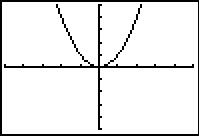
\includegraphics[width=1.8in]{./RelationsandFunctionsGraphics/Trans01.jpg} \;\;\;\;

&

\stackrel{\stackrel{\mbox{\tiny shift up $2$ units }}{\xrightarrow{\hspace{1in}}}}{\mbox{ \tiny add $2$ to each $y$-coordinate}} 

&

\;\;\;\; 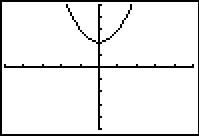
\includegraphics[width=1.8in]{./RelationsandFunctionsGraphics/Trans02.jpg} \\

y = f(x) = x^2 \;\;\;\; && \;\;\;\; y = g_{\mbox{\tiny$1$}}(x) = f(x) + 2 = x^2+2 \\

\end{array}\]



\[ \begin{array}{ccc}

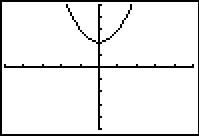
\includegraphics[width=1.8in]{./RelationsandFunctionsGraphics/Trans02.jpg}

&

\stackrel{\stackrel{\mbox{\tiny reflect across $x$-axis }}{\xrightarrow{\hspace{1in}}}}{\mbox{ \tiny multiply each $y$-coordinate by $-1$}} 

&

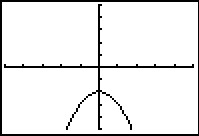
\includegraphics[width=1.8in]{./RelationsandFunctionsGraphics/Trans03.jpg} \\

y = g_{\mbox{\tiny$1$}}(x) = x^2+2&& y = g_{\mbox{\tiny$2$}}(x) = -g_{\mbox{\tiny$1$}}(x)= -x^2 -2 \\

\end{array}\]



\[ \begin{array}{ccc}

\, 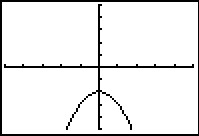
\includegraphics[width=1.8in]{./RelationsandFunctionsGraphics/Trans03.jpg} \;\;\;\,

&

\stackrel{\stackrel{\mbox{\tiny shift right $1$ unit }}{\xrightarrow{\hspace{1in}}}}{\mbox{ \tiny add $1$ to each $x$-coordinate}} 

&

\;\;\;\, 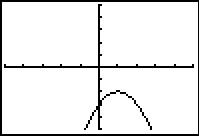
\includegraphics[width=1.8in]{./RelationsandFunctionsGraphics/Trans04.jpg} \\

\, y = g_{\mbox{\tiny$2$}}(x) = -x^2 -2 \;\;\;\, && \;\;\;\, y = g_{\mbox{\tiny$3$}}(x) = g_{\mbox{\tiny$2$}}(x-1) = -x^2+2x-3 \\

\end{array}\]


\[ \begin{array}{ccc}

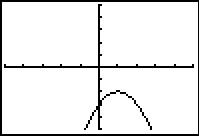
\includegraphics[width=1.8in]{./RelationsandFunctionsGraphics/Trans04.jpg}

&

\stackrel{\stackrel{\mbox{\tiny horizontal stretch by a factor of $2$ }}{\xrightarrow{\hspace{1.5in}}}}{\mbox{ \tiny multiply each $x$-coordinate by $2$}} 

&

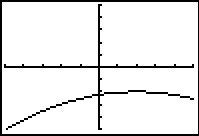
\includegraphics[width=1.8in]{./RelationsandFunctionsGraphics/Trans05.jpg} \\

y = g_{\mbox{\tiny$3$}}(x) = -x^2+2x-3 && y = g(x) = g_{\mbox{\tiny$3$}}\left(\frac{1}{2} x\right) = -\frac{1}{4}x^2+x-3 \\

\end{array}\]

\qed

\end{ex}

We have kept the viewing window the same in all of the graphs above.  This had the undesirable consequence of making the last graph look `incomplete' in that we cannot see the original shape of $f(x) = x^{2}$.  Altering the viewing window results in a more complete graph of the transformed function as seen below.

\smallskip

\begin{center}

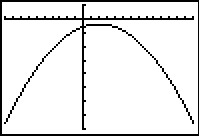
\includegraphics[width=1.8in]{./RelationsandFunctionsGraphics/Trans06.jpg} 

$y = g(x)$

\end{center}

\smallskip

This example brings our first chapter to a close.  In the chapters which lie ahead, be on the lookout for the concepts developed here to resurface as we study different families of functions.  

\newpage

\subsection{Exercises}

Suppose $(2,-3)$ is on the graph of $y = f(x)$.  In Exercises \ref{transformpointfirst} - \ref{transformpointlast}, use Theorem \ref{transformationsthm} to find a point on the graph of the given transformed function.

\begin{multicols}{3}
\begin{enumerate}

\item $y = f(x)+3$ \label{transformpointfirst}
\item $y = f(x+3)$
\item $y = f(x)-1$

\setcounter{HW}{\value{enumi}}
\end{enumerate}
\end{multicols}

\begin{multicols}{3}
\begin{enumerate}
\setcounter{enumi}{\value{HW}}

\item $y = f(x-1)$
\item $y = 3f(x)$
\item $y = f(3x)$

\setcounter{HW}{\value{enumi}}
\end{enumerate}
\end{multicols}

\begin{multicols}{3}
\begin{enumerate}
\setcounter{enumi}{\value{HW}}

\item $y = -f(x)$
\item $y = f(-x)$
\item $y = f(x-3)+1$

\setcounter{HW}{\value{enumi}}
\end{enumerate}
\end{multicols}

\begin{multicols}{3}
\begin{enumerate}
\setcounter{enumi}{\value{HW}}

\item $y = 2f(x+1)$
\item $y = 10 - f(x)$
\item $y = 3f(2x) - 1$

\setcounter{HW}{\value{enumi}}
\end{enumerate}
\end{multicols}

\begin{multicols}{3}
\begin{enumerate}
\setcounter{enumi}{\value{HW}}

\item $y = \frac{1}{2} f(4-x)$
\item $y = 5f(2x+1) + 3$
\item $y = 2f(1-x) -1$

\setcounter{HW}{\value{enumi}}
\end{enumerate}
\end{multicols}

\begin{multicols}{3}
\begin{enumerate}
\setcounter{enumi}{\value{HW}}

\item $y =f\left(\dfrac{7-2x}{4}\right)$
\item $y = \dfrac{f(3x) - 1}{2}$
\item $y = \dfrac{4-f(3x-1)}{7}$ \label{transformpointlast}

\setcounter{HW}{\value{enumi}}
\end{enumerate}
\end{multicols}

The complete graph of $y = f(x)$ is given below.  In Exercises \ref{transformgraphfirst} - \ref{transformgraphlast}, use it and Theorem \ref{transformationsthm} to graph the given transformed function.

\vspace{-.1in}
\begin{center}

\begin{mfpic}[15]{-5}{5}{-1}{5}
\axes
\arrow \reverse \arrow \polyline{(-4,4), (0,0), (4,4)}
\point[3pt]{(-2,2), (0,0), (2,2)}
\tlabel[cc](5,-0.25){\scriptsize $x$}
\tlabel[cc](0.25,5){\scriptsize $y$}
\tlabel[cc](-2.5,1.25){\scriptsize $(-2,2)$}
\tlabel[cc](0.75,-0.5){\scriptsize $(0,0)$}
\tlabel[cc](2.25,1.25){\scriptsize $(2,2)$}
\tcaption{The graph for Ex. \ref{transformgraphfirst} - \ref{transformgraphlast}}
\xmarks{-4,-3,-2,-1,2,3,4}
\ymarks{1,2,3,4}
\tlpointsep{5pt}
\scriptsize
\axislabels {x}{{$-4 \hspace{7pt}$} -4,{$-3 \hspace{7pt}$} -3, {$-2 \hspace{7pt}$} -2, {$-1 \hspace{7pt}$} -1, {$2$} 2,{$3$} 3,{$4$} 4}
\axislabels {y}{{$1$} 1, {$2$} 2, {$3$} 3, {$4$} 4}
\normalsize
\end{mfpic} 

\end{center}

\begin{multicols}{3}
\begin{enumerate}
\setcounter{enumi}{\value{HW}}

\item $y = f(x) + 1$ \label{transformgraphfirst}
\item $y = f(x) - 2$
\item $y = f(x+1)$

\setcounter{HW}{\value{enumi}}
\end{enumerate}
\end{multicols}

\begin{multicols}{3}
\begin{enumerate}
\setcounter{enumi}{\value{HW}}

\item $y = f(x - 2)$
\item $y = 2f(x)$
\item $y = f(2x)$

\setcounter{HW}{\value{enumi}}
\end{enumerate}
\end{multicols}

\begin{multicols}{3}
\begin{enumerate}
\setcounter{enumi}{\value{HW}}

\item $y = 2 - f(x)$
\item $y = f(2-x)$
\item $y = 2-f(2-x)$ \label{transformgraphlast}

\setcounter{HW}{\value{enumi}}
\end{enumerate}
\end{multicols}


\begin{enumerate}
\setcounter{enumi}{\value{HW}}

\item Some of the answers to Exercises \ref{transformgraphfirst} - \ref{transformgraphlast} above should be the same.  Which ones match up?  What properties of the graph of $y=f(x)$ contribute to the duplication?

\setcounter{HW}{\value{enumi}}
\end{enumerate}

\pagebreak

The complete graph of $y = f(x)$ is given below.  In Exercises \ref{transsecondgraphfirst} - \ref{transsecondgraphlast}, use it and Theorem \ref{transformationsthm} to graph the given transformed function.

\vspace{-.1in}
\begin{center}

\begin{mfpic}[15]{-5}{5}{-5}{5}
\axes
\polyline{(-2,0), (0,4), (2,0), (4,-2)}
\point[3pt]{(-2,0), (0,4), (2,0), (4,-2)}
\tlabel[cc](5,-0.25){\scriptsize $x$}
\tlabel[cc](0.25,5){\scriptsize $y$}
\tlabel[cc](-2.25,-1.25){\scriptsize $(-2,0)$}
\tlabel[cc](1,4){\scriptsize $(0,4)$}
\tlabel[cc](2,-1.25){\scriptsize $(2,0)$}
\tlabel[cc](4,-2.5){\scriptsize $(4,-2)$}
\tcaption{The graph for Ex. \ref{transsecondgraphfirst} - \ref{transsecondgraphlast}}
\xmarks{-4,-3,-2,-1,1,2,3,4}
\ymarks{-4,-3,-2,-1,1,2,3,4}
\tlpointsep{5pt}
\scriptsize
\axislabels {x}{{$-4 \hspace{7pt}$} -4,{$-3 \hspace{7pt}$} -3, {$-1 \hspace{7pt}$} -1,{$1$} 1,{$3$} 3,{$4$} 4}
\axislabels {y}{{$-4$} -4,{$-3$} -3,{$-2$} -2, {$-1$} -1, {$1$} 1, {$2$} 2, {$3$} 3, {$4$} 4}
\normalsize
\end{mfpic} 

\end{center}

\begin{multicols}{3}
\begin{enumerate}
\setcounter{enumi}{\value{HW}}

\item  $y = f(x) - 1$ \label{transsecondgraphfirst}
\item  $y = f(x + 1)$
\item  $y = \frac{1}{2} f(x)$

\setcounter{HW}{\value{enumi}}
\end{enumerate}
\end{multicols}

\begin{multicols}{3}
\begin{enumerate}
\setcounter{enumi}{\value{HW}}

\item  $y = f(2x)$
\item  $y = - f(x)$
\item  $y = f(-x)$

\setcounter{HW}{\value{enumi}}
\end{enumerate}
\end{multicols}

\begin{multicols}{3}
\begin{enumerate}
\setcounter{enumi}{\value{HW}}

\item  $y = f(x+1) - 1$
\item  $y = 1 - f(x)$
\item  $y = \frac{1}{2}f(x+1)-1$ \label{transsecondgraphlast}

\setcounter{HW}{\value{enumi}}
\end{enumerate}
\end{multicols}

The complete graph of $y = f(x)$ is given below.  In Exercises \ref{transthirdgraphfirst} - \ref{transthirdgraphlast}, use it and Theorem \ref{transformationsthm} to graph the given transformed function.

\vspace{-.1in}
\begin{center}

\begin{mfpic}[20]{-4}{4}{-1.5}{4}
\point[3pt]{(-3,0),(3,0),(0,3)}
\parafcn{0,3.14159,0.1}{(3*cos(t), 3*sin(t))}
\tlabel[cc](-3,-1){\small $\left(-3, 0 \right)$}
\tlabel[cc](0.8,3.3){\small $\left(0, 3 \right)$}
\tlabel[cc](3,-1){\small $\left(3, 0 \right)$}
\axes
\tlabel[cc](4,-0.5){\scriptsize $x$}
\tlabel[cc](0.5,4){\scriptsize $y$}
\tcaption{The graph for Ex. \ref{transthirdgraphfirst} - \ref{transthirdgraphlast}}
\xmarks{-3,-2,-1,1,2,3}
\ymarks{-1,1,2,3}
\tlpointsep{5pt}
\scriptsize
\axislabels {x}{{$-3 \hspace{7pt}$} -3, {$-2 \hspace{7pt}$} -2, {$-1 \hspace{7pt}$} -1, {$1$} 1, {$2$} 2, {$3$} 3}
\axislabels {y}{{$-1$} -1, {$1$} 1, {$2$} 2, {$3$} 3}
\normalsize
\end{mfpic}

\end{center}

\begin{multicols}{3}
\begin{enumerate}
\setcounter{enumi}{\value{HW}}

\item $g(x) = f(x) + 3$ \label{transthirdgraphfirst}
\item $h(x) = f(x) - \frac{1}{2}$
\item $j(x) = f\left(x - \frac{2}{3}\right)$

\setcounter{HW}{\value{enumi}}
\end{enumerate}
\end{multicols}

\begin{multicols}{3}
\begin{enumerate}
\setcounter{enumi}{\value{HW}}

\item $a(x) = f(x + 4)$
\item $b(x) = f(x + 1) - 1$ 
\item $c(x) = \frac{3}{5}f(x)$


\setcounter{HW}{\value{enumi}}
\end{enumerate}
\end{multicols}

\begin{multicols}{3}
\begin{enumerate}
\setcounter{enumi}{\value{HW}}


\item $d(x) = -2f(x)$
\item $k(x) = f\left(\frac{2}{3}x\right)$
\item $m(x) = -\frac{1}{4}f(3x)$

\setcounter{HW}{\value{enumi}}
\end{enumerate}
\end{multicols}

\begin{multicols}{3}
\begin{enumerate}
\setcounter{enumi}{\value{HW}}

\item $n(x) = 4f(x - 3) - 6$
\item $p(x) = 4 + f(1 - 2x)$
\item $q(x) = -\frac{1}{2}f\left(\frac{x + 4}{2}\right) - 3$ \label{transthirdgraphlast}

\setcounter{HW}{\value{enumi}}
\end{enumerate}
\end{multicols}

\pagebreak

The complete graph of $y = S(x)$ is given below. 

\vspace{-.1in}
\begin{center}

\begin{mfpic}[20]{-3}{3}{-4}{4}
\axes
\function{-2,2,0.1}{3*sin(1.570796327*x)}
\point[3pt]{(-2,0), (-1,-3), (0,0), (1,3), (2,0)}
\tlabel[cc](3,-0.25){\scriptsize $x$}
\tlabel[cc](0.25,4){\scriptsize $y$}
\tlabel[cc](-2,0.5){\scriptsize $(-2,0)$}
\tlabel[cc](-1,-3.5){\scriptsize $(-1,-3)$}
\tlabel[cc](0.5,0.25){\scriptsize $(0,0)$}
\tlabel[cc](1,3.5){\scriptsize $(1,3)$}
\tlabel[cc](2,-0.5){\scriptsize $(2,0)$}
\tcaption{The graph of $y=S(x)$}
\xmarks{-2,-1,1,2}
\ymarks{-3,-2,-1,1,2,3}
\tlpointsep{5pt}
\scriptsize
\axislabels {x}{{$-2 \hspace{7pt}$} -2,{$-1 \hspace{7pt}$} -1,{$1$} 1}
\axislabels {y}{{$-3$} -3,{$-2$} -2, {$-1$} -1, {$1$} 1, {$2$} 2, {$3$} 3}
\normalsize
\end{mfpic} 

\end{center}

The purpose of Exercises \ref{transformsinegraphfirst} - \ref{transformsinegraphlast} is to graph $y = \frac{1}{2}S(-x+1) + 1$ by graphing each transformation, one step at a time.

\begin{multicols}{2}
\begin{enumerate}
\setcounter{enumi}{\value{HW}}

\item $y = S_{\text{\tiny $1$}}(x) = S(x + 1)$ \label{transformsinegraphfirst}
\item  $y = S_{\text{\tiny $2$}}(x) =  S_{\text{\tiny $1$}}(-x) = S(-x + 1)$

\setcounter{HW}{\value{enumi}}
\end{enumerate}
\end{multicols}

\begin{multicols}{2}
\begin{enumerate}
\setcounter{enumi}{\value{HW}}

\item  $y = S_{\text{\tiny $3$}}(x) = \frac{1}{2}  S_{\text{\tiny $2$}}(x) =  \frac{1}{2}S(-x+1)$
\item  $y = S_{\text{\tiny $4$}}(x) = S_{\text{\tiny $3$}}(x) + 1 = \frac{1}{2}S(-x+1) + 1$ \label{transformsinegraphlast}

\setcounter{HW}{\value{enumi}}
\end{enumerate}
\end{multicols}

Let $f(x) = \sqrt{x}$.  Find a formula for a function $g$ whose graph is obtained from $f$ from the given sequence of transformations. 

\begin{enumerate}
\setcounter{enumi}{\value{HW}}


\item  (1) shift right 2 units; (2) shift down 3 units

\item  (1) shift down 3 units; (2) shift right 2 units

\item  (1) reflect across the $x$-axis; (2) shift up 1 unit

\item  (1) shift up 1 unit; (2) reflect across the $x$-axis

\item  (1) shift left 1 unit; (2) reflect across the $y$-axis; (3) shift up 2 units

\item  (1) reflect across the $y$-axis;  (2) shift left 1 unit;  (3) shift up 2 units

\item  (1) shift left 3 units; (2) vertical stretch by a factor of 2; (3) shift down 4 units

\item  (1) shift left 3 units; (2) shift down 4 units; (3) vertical stretch by a factor of 2

\item  (1) shift right 3 units; (2) horizontal shrink by a factor of 2; (3) shift up 1 unit

\item  (1) horizontal shrink by a factor of 2; (2) shift right 3 units; (3) shift up 1 unit


\setcounter{HW}{\value{enumi}}
\end{enumerate}


\begin{enumerate}
\setcounter{enumi}{\value{HW}}

\item The graph of $y = f(x) = \sqrt[3]{x}$ is given below on the left and the graph of $y = g(x)$ is given on the right. Find a formula for $g$ based on transformations of the graph of $f$.  Check your answer by confirming that the points shown on the graph of $g$ satisfy the equation $y = g(x)$.

\[ \begin{array}{cc}

\begin{mfpic}[10]{-12}{9}{-6}{6}
\point[3pt]{(0,0), (-1, -1), (1, 1), (-8, -2), (8, 2)}
\axes
\tlabel[cc](9,-0.5){\scriptsize $x$}
\tlabel[cc](0.5,6){\scriptsize $y$}
\xmarks{-11 step 1 until 8}
\ymarks{-5 step 1 until 5}
\tlpointsep{4pt}
\axislabels {x}{{\tiny $-11 \hspace{6pt}$} -11, {\tiny $-10 \hspace{6pt}$} -10, {\tiny $-9 \hspace{6pt}$} -9, {\tiny $-8 \hspace{6pt}$} -8, {\tiny $-7 \hspace{6pt}$} -7, {\tiny $-6 \hspace{6pt}$} -6, {\tiny $-5 \hspace{6pt}$} -5, {\tiny $-4 \hspace{6pt}$} -4, {\tiny $-3 \hspace{6pt}$} -3, {\tiny $-2 \hspace{6pt}$} -2, {\tiny $-1 \hspace{6pt}$} -1, {\tiny $1$} 1, {\tiny $2$} 2, {\tiny $3$} 3, {\tiny $4$} 4, {\tiny $5$} 5, {\tiny $6$} 6, {\tiny $7$} 7, {\tiny $8$} 8}
\axislabels {y}{{\tiny $-5$} -5, {\tiny $-4$} -4, {\tiny $-3$} -3, {\tiny $-2$} -2, {\tiny $-1$} -1, {\tiny $1$} 1, {\tiny $2$} 2, {\tiny $3$} 3, {\tiny $4$} 4, {\tiny $5$} 5}
\arrow \reverse \arrow \parafcn{-2.1,2.1,0.1}{(t**3,t)}
\tcaption{\scriptsize $y = \sqrt[3]{x}$}
\end{mfpic}

&

\begin{mfpic}[10]{-12}{9}{-6}{6}
\point[3pt]{(-11,3), (-4,1), (-3,-1), (-2,-3), (5,-5)}
\axes
\tlabel[cc](9,-0.5){\scriptsize $x$}
\tlabel[cc](0.5,6){\scriptsize $y$}
\xmarks{-11 step 1 until 8}
\ymarks{-5 step 1 until 5}
\tlpointsep{4pt}
\axislabels {x}{{\tiny $-11 \hspace{6pt}$} -11, {\tiny $-10 \hspace{6pt}$} -10, {\tiny $-9 \hspace{6pt}$} -9, {\tiny $-8 \hspace{6pt}$} -8, {\tiny $-7 \hspace{6pt}$} -7, {\tiny $-6 \hspace{6pt}$} -6, {\tiny $-5 \hspace{6pt}$} -5, {\tiny $-4 \hspace{6pt}$} -4, {\tiny $-3 \hspace{6pt}$} -3, {\tiny $-2 \hspace{6pt}$} -2, {\tiny $-1 \hspace{6pt}$} -1, {\tiny $1$} 1, {\tiny $2$} 2, {\tiny $3$} 3, {\tiny $4$} 4, {\tiny $5$} 5, {\tiny $6$} 6, {\tiny $7$} 7, {\tiny $8$} 8}
\axislabels {y}{{\tiny $-5$} -5, {\tiny $-4$} -4, {\tiny $-3$} -3, {\tiny $-2$} -2, {\tiny $-1$} -1, {\tiny $1$} 1, {\tiny $2$} 2, {\tiny $3$} 3, {\tiny $4$} 4, {\tiny $5$} 5}
\arrow \reverse \arrow \parafcn{-2.1,2.1,0.1}{((t**3 - 3),((-2*t) - 1))}
\tcaption{\scriptsize $y = g(x)$}
\end{mfpic}

\end{array} \]

\item For many common functions, the properties of Algebra make a horizontal scaling the same as a vertical scaling by (possibly) a different factor.  For example, we stated earlier that $\sqrt{9x} = 3\sqrt{x}$.  With the help of your classmates, find the equivalent vertical scaling produced by the horizontal scalings $y = (2x)^{3}, \, y = |5x|, \, y = \sqrt[3]{27x} \, $ and $\, y = \left(\frac{1}{2} x\right)^{2}$.  What about $y = (-2x)^{3}, \, y = |-5x|, \, y = \sqrt[3]{-27x}\, $ and $\, y = \left(-\frac{1}{2} x\right)^{2}$?

\item We mentioned earlier in the section that, in general, the order in which transformations are applied matters, yet in our first example with two transformations the order did not matter. (You could perform the shift to the left followed by the shift down or you could shift down and then left to achieve the same result.)  With the help of your classmates, determine the situations in which order does matter and those in which it does not.

\item What happens if you reflect an even function across the $y$-axis?  
\item What happens if you reflect an odd function across the $y$-axis?   
\item What happens if you reflect an even function across the $x$-axis?  
\item What happens if you reflect an odd function across the $x$-axis?  
\item How would you describe symmetry about the origin in terms of reflections?

\item As we saw in Example \ref{graphingcalctrans}, the viewing window on the graphing calculator affects how we see the transformations done to a graph.  Using two different calculators, find viewing windows so that $f(x) = x^{2}$ on the one calculator looks like $g(x) = 3x^{2}$ on the other.

\end{enumerate}

\newpage

\subsection{Answers}

\begin{multicols}{3}
\begin{enumerate}

\item $(2,0)$
\item $(-1,-3)$
\item $(2,-4)$

\setcounter{HW}{\value{enumi}}
\end{enumerate}
\end{multicols}

\begin{multicols}{3}
\begin{enumerate}
\setcounter{enumi}{\value{HW}}

\item $(3,-3)$
\item $(2,-9)$
\item $\left(\frac{2}{3}, -3\right)$

\setcounter{HW}{\value{enumi}}
\end{enumerate}
\end{multicols}

\begin{multicols}{3}
\begin{enumerate}
\setcounter{enumi}{\value{HW}}

\item $(2,3)$
\item $(-2,-3)$
\item $(5,-2)$

\setcounter{HW}{\value{enumi}}
\end{enumerate}
\end{multicols}

\begin{multicols}{3}
\begin{enumerate}
\setcounter{enumi}{\value{HW}}

\item $(1,-6)$
\item $(2,13)$
\item $y = (1,-10)$

\setcounter{HW}{\value{enumi}}
\end{enumerate}
\end{multicols}

\begin{multicols}{3}
\begin{enumerate}
\setcounter{enumi}{\value{HW}}

\item $\left(2, -\frac{3}{2}\right)$
\item $\left(\frac{1}{2}, -12 \right)$
\item $(-1,-7)$

\setcounter{HW}{\value{enumi}}
\end{enumerate}
\end{multicols}

\begin{multicols}{3}
\begin{enumerate}
\setcounter{enumi}{\value{HW}}

\item $\left(-\frac{1}{2}, -3\right)$
\item $\left(\frac{2}{3}, -2 \right)$
\item $(1,1)$

\setcounter{HW}{\value{enumi}}
\end{enumerate}
\end{multicols}

\begin{multicols}{2}
\begin{enumerate}
\setcounter{enumi}{\value{HW}}

\item $y = f(x) + 1$

\begin{mfpic}[15]{-5}{5}{-1}{5}
\axes
\arrow \reverse \arrow \polyline{(-4,5), (0,1), (4,5)}
\point[3pt]{(-2,3), (0,1), (2,3)}
\tlabel[cc](5,-0.25){\scriptsize $x$}
\tlabel[cc](0.25,5){\scriptsize $y$}
\tlabel[cc](-2.5,2.25){\scriptsize $(-2,3)$}
\tlabel[cc](0.75,0.5){\scriptsize $(0,1)$}
\tlabel[cc](2.25,2.25){\scriptsize $(2,3)$}
\xmarks{-4,-3,-2,-1,1,2,3,4}
\ymarks{1,2,3,4}
\tlpointsep{5pt}
\scriptsize
\axislabels {x}{{$-4 \hspace{7pt}$} -4,{$-3 \hspace{7pt}$} -3, {$-2 \hspace{7pt}$} -2, {$-1 \hspace{7pt}$} -1, {$1$} 1, {$2$} 2,{$3$} 3,{$4$} 4}
\axislabels {y}{{$1$} 1, {$2$} 2, {$3$} 3, {$4$} 4}
\normalsize
\end{mfpic} 

\vfill

\columnbreak

\item $y = f(x) - 2$

\begin{mfpic}[15]{-5}{5}{-3}{3}
\axes
\arrow \reverse \arrow \polyline{(-4,2), (0,-2), (4,2)}
\point[3pt]{(-2,0), (0,-2), (2,0)}
\tlabel[cc](5,-0.25){\scriptsize $x$}
\tlabel[cc](0.25,3){\scriptsize $y$}
\tlabel[cc](-2.5,-0.75){\scriptsize $(-2,2)$}
\tlabel[cc](0.75,-2.5){\scriptsize $(0,-2)$}
\tlabel[cc](2.25,-0.75){\scriptsize $(2,2)$}
\xmarks{-4,-3,-2,-1,1,2,3,4}
\ymarks{-2,-1,1,2}
\tlpointsep{5pt}
\scriptsize
\axislabels {x}{{$-4 \hspace{7pt}$} -4, {$-1 \hspace{7pt}$} -1, {$1$} 1,{$4$} 4}
\axislabels {y}{{$-2$} -2, {$-1$} -1, {$1$} 1, {$2$} 2}
\normalsize
\end{mfpic} 

\setcounter{HW}{\value{enumi}}
\end{enumerate}
\end{multicols}

\begin{multicols}{2}
\begin{enumerate}
\setcounter{enumi}{\value{HW}}

\item $y = f(x+1)$

\begin{mfpic}[15]{-6}{4}{-1}{5}
\axes
\arrow \reverse \arrow \polyline{(-5,4), (-1,0), (3,4)}
\point[3pt]{(-3,2), (-1,0), (1,2)}
\tlabel[cc](4,-0.25){\scriptsize $x$}
\tlabel[cc](0.25,5){\scriptsize $y$}
\tlabel[cc](-3.5,1.25){\scriptsize $(-3,2)$}
\tlabel[cc](-1,-0.5){\scriptsize $(-1,0)$}
\tlabel[cc](1.25,1.25){\scriptsize $(1,2)$}
\xmarks{-5,-4,-3,-2,-1,1,2,3}
\ymarks{1,2,3,4}
\tlpointsep{5pt}
\scriptsize
\axislabels {x}{{$-5 \hspace{7pt}$} -5,{$-4 \hspace{7pt}$} -4,{$-3 \hspace{7pt}$} -3, {$1$} 1, {$2$} 2,{$3$} 3}
\axislabels {y}{{$1$} 1, {$2$} 2, {$3$} 3, {$4$} 4}
\normalsize
\end{mfpic} 

\vfill

\columnbreak

\item $y = f(x - 2)$

\begin{mfpic}[15]{-3}{7}{-1}{5}
\axes
\arrow \reverse \arrow \polyline{(-2,4), (2,0), (6,4)}
\point[3pt]{(0,2), (2,0), (4,2)}
\tlabel[cc](7,-0.25){\scriptsize $x$}
\tlabel[cc](0.25,5){\scriptsize $y$}
\tlabel[cc](0.75,2){\scriptsize $(0,2)$}
\tlabel[cc](2,-0.5){\scriptsize $(2,0)$}
\tlabel[cc](3,2){\scriptsize $(4,2)$}
\xmarks{-2,-1,1,2,3,4,5,6}
\ymarks{1,2,3,4}
\tlpointsep{5pt}
\scriptsize
\axislabels {x}{{$-2 \hspace{7pt}$} -2, {$-1 \hspace{7pt}$} -1, {$3$} 3,{$4$} 4,{$5$} 5,{$6$} 6}
\axislabels {y}{{$1$} 1, {$2$} 2,  {$4$} 4}
\normalsize
\end{mfpic} 

\setcounter{HW}{\value{enumi}}
\end{enumerate}
\end{multicols}

\begin{multicols}{2}
\begin{enumerate}
\setcounter{enumi}{\value{HW}}


\item $y = 2f(x)$

\begin{mfpic}[15]{-5}{5}{-1}{5}
\axes
\arrow \reverse \arrow \polyline{(-2.5,5), (0,0), (2.5,5)}
\point[3pt]{(-2,4), (0,0), (2,4)}
\tlabel[cc](5,-0.25){\scriptsize $x$}
\tlabel[cc](0.25,5){\scriptsize $y$}
\tlabel[cc](-2.75,3.5){\scriptsize $(-2,4)$}
\tlabel[cc](0.75,-0.5){\scriptsize $(0,0)$}
\tlabel[cc](2.5,3.5){\scriptsize $(2,4)$}
\xmarks{-4,-3,-2,-1,2,3,4}
\ymarks{1,2,3,4}
\tlpointsep{5pt}
\scriptsize
\axislabels {x}{{$-4 \hspace{7pt}$} -4,{$-3 \hspace{7pt}$} -3, {$-2 \hspace{7pt}$} -2, {$-1 \hspace{7pt}$} -1, {$2$} 2,{$3$} 3,{$4$} 4}
\axislabels {y}{{$1$} 1, {$2$} 2, {$3$} 3, {$4$} 4}
\normalsize
\end{mfpic} 


\vfill

\columnbreak

\item $y = f(2x)$

\begin{mfpic}[15]{-5}{5}{-1}{5}
\axes
\arrow \reverse \arrow \polyline{(-2.5,5), (0,0), (2.5,5)}
\point[3pt]{(-1,2), (0,0), (1,2)}
\tlabel[cc](5,-0.25){\scriptsize $x$}
\tlabel[cc](0.25,5){\scriptsize $y$}
\tlabel[cc](-1.75,1.5){\scriptsize $(-1,2)$}
\tlabel[cc](0.75,-0.5){\scriptsize $(0,0)$}
\tlabel[cc](1.5,1.5){\scriptsize $(1,2)$}
\xmarks{-4,-3,-2,-1,2,3,4}
\ymarks{1,2,3,4}
\tlpointsep{5pt}
\scriptsize
\axislabels {x}{{$-4 \hspace{7pt}$} -4,{$-3 \hspace{7pt}$} -3, {$-2 \hspace{7pt}$} -2, {$-1 \hspace{7pt}$} -1, {$2$} 2,{$3$} 3,{$4$} 4}
\axislabels {y}{{$1$} 1, {$2$} 2, {$3$} 3, {$4$} 4}
\normalsize
\end{mfpic} 


\setcounter{HW}{\value{enumi}}
\end{enumerate}
\end{multicols}

\begin{multicols}{2}
\begin{enumerate}
\setcounter{enumi}{\value{HW}}

\item $y = 2 - f(x)$

\begin{mfpic}[15]{-5}{5}{-2}{3}
\axes
\arrow \reverse \arrow \polyline{(-4,-2), (0,2), (4,-2)}
\point[3pt]{(-2,0), (0,2), (2,0)}
\tlabel[cc](5,-0.25){\scriptsize $x$}
\tlabel[cc](0.25,3){\scriptsize $y$}
\tlabel[cc](-1.25,-0.5){\scriptsize $(-2,0)$}
\tlabel[cc](0.75,2){\scriptsize $(0,2)$}
\tlabel[cc](1.5,-0.5){\scriptsize $(2,0)$}
\xmarks{-4,-3,-2,-1,2,3,4}
\ymarks{-1,1,2}
\tlpointsep{5pt}
\scriptsize
\axislabels {x}{{$-4 \hspace{7pt}$} -4,{$-3 \hspace{7pt}$} -3,  {$3$} 3,{$4$} 4}
\axislabels {y}{{$1$} 1, {$2$} 2}
\normalsize
\end{mfpic} 

\vfill

\columnbreak

\item $y = f(2-x)$

\begin{mfpic}[15]{-3}{7}{-1}{5}
\axes
\arrow \reverse \arrow \polyline{(-2,4), (2,0), (6,4)}
\point[3pt]{(0,2), (2,0), (4,2)}
\tlabel[cc](7,-0.25){\scriptsize $x$}
\tlabel[cc](0.25,5){\scriptsize $y$}
\tlabel[cc](0.75,2){\scriptsize $(0,2)$}
\tlabel[cc](2,-0.5){\scriptsize $(2,0)$}
\tlabel[cc](3,2){\scriptsize $(4,2)$}
\xmarks{-2,-1,1,2,3,4,5,6}
\ymarks{1,2,3,4}
\tlpointsep{5pt}
\scriptsize
\axislabels {x}{{$-2 \hspace{7pt}$} -2, {$-1 \hspace{7pt}$} -1, {$3$} 3,{$4$} 4,{$5$} 5,{$6$} 6}
\axislabels {y}{{$1$} 1, {$2$} 2, {$4$} 4}
\normalsize
\end{mfpic} 

\setcounter{HW}{\value{enumi}}
\end{enumerate}
\end{multicols}

\begin{multicols}{2}
\begin{enumerate}
\setcounter{enumi}{\value{HW}}

\item $y = 2-f(2-x)$

\begin{mfpic}[15]{-3}{7}{-1}{5}
\axes
\arrow \reverse \arrow \polyline{(-2,-2), (2,2), (6,-2)}
\point[3pt]{(0,0), (2,2), (4,0)}
\tlabel[cc](7,-0.25){\scriptsize $x$}
\tlabel[cc](0.25,5){\scriptsize $y$}
\tlabel[cc](0.75,-0.5){\scriptsize $(0,0)$}
\tlabel[cc](2,2.5){\scriptsize $(2,2)$}
\tlabel[cc](3.5,-0.5){\scriptsize $(4,0)$}
\xmarks{-2,-1,1,2,3,4,5,6}
\ymarks{1,2,3,4}
\tlpointsep{5pt}
\scriptsize
\axislabels {x}{{$-2 \hspace{7pt}$} -2, {$-1 \hspace{7pt}$} -1, {$2$} 2,{$5$} 5, {$6$} 6}
\axislabels {y}{{$1$} 1, {$2$} 2, {$3$} 3, {$4$} 4}
\normalsize
\end{mfpic} 

\vfill

\columnbreak

\addtocounter{enumi}{1}

\item  $y = f(x) - 1$

\begin{mfpic}[15]{-5}{5}{-5}{5}
\axes
\polyline{(-2,-1), (0,3), (2,-1), (4,-3)}
\point[3pt]{(-2,-1), (0,3), (2,-1), (4,-3)}
\tlabel[cc](5,-0.25){\scriptsize $x$}
\tlabel[cc](0.25,5){\scriptsize $y$}
\tlabel[cc](-2.25,-1.5){\scriptsize $(-2,-1)$}
\tlabel[cc](1,3){\scriptsize $(0,3)$}
\tlabel[cc](1,-1.5){\scriptsize $(2,-1)$}
\tlabel[cc](4,-3.5){\scriptsize $(4,-3)$}
\xmarks{-4,-3,-2,-1,1,2,3,4}
\ymarks{-4,-3,-2,-1,1,2,3,4}
\tlpointsep{5pt}
\scriptsize
\axislabels {x}{{$-4 \hspace{7pt}$} -4,{$-3 \hspace{7pt}$} -3, {$-1 \hspace{7pt}$} -1,{$-2 \hspace{7pt}$} -2,{$1$} 1,{$2$} 2,{$3$} 3,{$4$} 4}
\axislabels {y}{{$-4$} -4,{$-3$} -3,{$-2$} -2, {$-1$} -1, {$1$} 1, {$2$} 2, {$3$} 3, {$4$} 4}
\normalsize
\end{mfpic} 


\setcounter{HW}{\value{enumi}}
\end{enumerate}
\end{multicols}

\begin{multicols}{2}
\begin{enumerate}
\setcounter{enumi}{\value{HW}}

\item  $y = f(x + 1)$

\begin{mfpic}[15]{-5}{5}{-5}{5}
\axes
\polyline{(-3,0), (-1,4), (1,0), (3,-2)}
\point[3pt]{(-3,0), (-1,4), (1,0), (3,-2)}
\tlabel[cc](5,-0.25){\scriptsize $x$}
\tlabel[cc](0.25,5){\scriptsize $y$}
\tlabel[cc](-3.25,-1.25){\scriptsize $(-3,0)$}
\tlabel[cc](-3,4){\scriptsize $(-1,4)$}
\tlabel[cc](1,-1.25){\scriptsize $(1,0)$}
\tlabel[cc](3,-2.5){\scriptsize $(3,-2)$}
\xmarks{-4,-3,-2,-1,1,2,3,4}
\ymarks{-4,-3,-2,-1,1,2,3,4}
\tlpointsep{5pt}
\scriptsize
\axislabels {x}{{$-4 \hspace{7pt}$} -4,{$-3 \hspace{7pt}$} -3, {$-1 \hspace{7pt}$} -1,{$-2 \hspace{7pt}$} -2,{$1$} 1,{$2$} 2,{$3$} 3,{$4$} 4}
\axislabels {y}{{$-4$} -4,{$-3$} -3,{$-2$} -2, {$-1$} -1, {$1$} 1, {$2$} 2, {$3$} 3, {$4$} 4}
\normalsize
\end{mfpic} 

\vfill

\columnbreak

\item  $y = \frac{1}{2} f(x)$

\begin{mfpic}[15]{-5}{5}{-5}{5}
\axes
\polyline{(-2,0), (0,2), (2,0), (4,-1)}
\point[3pt]{(-2,0), (0,2), (2,0), (4,-1)}
\tlabel[cc](5,-0.25){\scriptsize $x$}
\tlabel[cc](0.25,5){\scriptsize $y$}
\tlabel[cc](-2.25,-1.25){\scriptsize $(-2,0)$}
\tlabel[cc](1,2){\scriptsize $(0,2)$}
\tlabel[cc](2,-1.25){\scriptsize $(2,0)$}
\tlabel[cc](4,-1.5){\scriptsize $(4,-1)$}
\xmarks{-4,-3,-2,-1,1,2,3,4}
\ymarks{-4,-3,-2,-1,1,2,3,4}
\tlpointsep{5pt}
\scriptsize
\axislabels {x}{{$-4 \hspace{7pt}$} -4,{$-3 \hspace{7pt}$} -3, {$-1 \hspace{7pt}$} -1,{$1$} 1,{$3$} 3,{$4$} 4}
\axislabels {y}{{$-4$} -4,{$-3$} -3,{$-2$} -2, {$-1$} -1, {$1$} 1, {$2$} 2, {$3$} 3, {$4$} 4}
\normalsize
\end{mfpic} 

\setcounter{HW}{\value{enumi}}
\end{enumerate}
\end{multicols}

\pagebreak

\begin{multicols}{2}
\begin{enumerate}
\setcounter{enumi}{\value{HW}}
\item  $y = f(2x)$

\begin{mfpic}[15]{-5}{5}{-5}{5}
\axes
\polyline{(-1,0), (0,4), (1,0), (2,-2)}
\point[3pt]{(-1,0), (0,4), (1,0), (2,-2)}
\tlabel[cc](5,-0.25){\scriptsize $x$}
\tlabel[cc](0.25,5){\scriptsize $y$}
\tlabel[cc](-1,-0.75){\scriptsize $(-1,0)$}
\tlabel[cc](1,4){\scriptsize $(0,4)$}
\tlabel[cc](1.75,0.5){\scriptsize $(1,0)$}
\tlabel[cc](2,-2.5){\scriptsize $(2,-2)$}
\xmarks{-4,-3,-2,-1,1,2,3,4}
\ymarks{-4,-3,-2,-1,1,2,3,4}
\tlpointsep{5pt}
\scriptsize
\axislabels {x}{{$-4 \hspace{7pt}$} -4,{$-3 \hspace{7pt}$} -3, {$-2 \hspace{7pt}$} -2,{$2$} 2,{$3$} 3,{$4$} 4}
\axislabels {y}{{$-4$} -4,{$-3$} -3,{$-2$} -2, {$1$} 1, {$2$} 2, {$3$} 3, {$4$} 4}
\normalsize
\end{mfpic} 


\vfill

\columnbreak

\item  $y = - f(x)$

\begin{mfpic}[15]{-5}{5}{-5}{5}
\axes
\polyline{(-2,0), (0,-4), (2,0), (4,2)}
\point[3pt]{(-2,0), (0,-4), (2,0), (4,2)}
\tlabel[cc](5,-0.25){\scriptsize $x$}
\tlabel[cc](0.25,5){\scriptsize $y$}
\tlabel[cc](-2.25,.75){\scriptsize $(-2,0)$}
\tlabel[cc](1.25,-4){\scriptsize $(0,-4)$}
\tlabel[cc](1.75,.75){\scriptsize $(2,0)$}
\tlabel[cc](4,2.5){\scriptsize $(4,2)$}
\xmarks{-4,-3,-2,-1,1,2,3,4}
\ymarks{-4,-3,-2,-1,1,2,3,4}
\tlpointsep{5pt}
\scriptsize
\axislabels {x}{{$-4 \hspace{7pt}$} -4,{$-3 \hspace{7pt}$} -3, {$-1 \hspace{7pt}$} -1,{$-2 \hspace{7pt}$} -2,{$1$} 1,{$2$} 2,{$3$} 3,{$4$} 4}
\axislabels {y}{{$-4$} -4,{$-3$} -3,{$-2$} -2, {$-1$} -1, {$1$} 1, {$2$} 2, {$3$} 3, {$4$} 4}
\normalsize
\end{mfpic} 

\setcounter{HW}{\value{enumi}}
\end{enumerate}
\end{multicols}

\begin{multicols}{2}
\begin{enumerate}
\setcounter{enumi}{\value{HW}}

\item  $y = f(-x)$

\begin{mfpic}[15]{-5}{5}{-5}{5}
\axes
\polyline{(2,0), (0,4), (-2,0), (-4,-2)}
\point[3pt]{(2,0), (0,4), (-2,0), (-4,-2)}
\tlabel[cc](5,-0.25){\scriptsize $x$}
\tlabel[cc](0.25,5){\scriptsize $y$}
\tlabel[cc](2.25,-1.25){\scriptsize $(2,0)$}
\tlabel[cc](1,4){\scriptsize $(0,4)$}
\tlabel[cc](-2,-1.25){\scriptsize $(-2,0)$}
\tlabel[cc](-4,-2.5){\scriptsize $(-4,-2)$}
\xmarks{-4,-3,-2,-1,1,2,3,4}
\ymarks{-4,-3,-2,-1,1,2,3,4}
\tlpointsep{5pt}
\scriptsize
\axislabels {x}{{$-4 \hspace{7pt}$} -4,{$-3 \hspace{7pt}$} -3, {$-1 \hspace{7pt}$} -1,{$1$} 1,{$3$} 3,{$4$} 4}
\axislabels {y}{{$-4$} -4,{$-3$} -3,{$-2$} -2, {$-1$} -1, {$1$} 1, {$2$} 2, {$3$} 3, {$4$} 4}
\normalsize
\end{mfpic} 


\vfill
\columnbreak

\item  $y = f(x+1) - 1$

\begin{mfpic}[15]{-5}{5}{-5}{5}
\axes
\polyline{(-3,-1), (-1,3), (1,-1), (3,-3)}
\point[3pt]{(-3,-1), (-1,3), (1,-1), (3,-3)}
\tlabel[cc](5,-0.25){\scriptsize $x$}
\tlabel[cc](0.25,5){\scriptsize $y$}
\tlabel[cc](-3.25,-2.25){\scriptsize $(-3,-1)$}
\tlabel[cc](-3,3){\scriptsize $(-1,3)$}
\tlabel[cc](2.5,-1){\scriptsize $(1,-1)$}
\tlabel[cc](3,-3.5){\scriptsize $(3,-3)$}
\xmarks{-4,-3,-2,-1,1,2,3,4}
\ymarks{-4,-3,-2,-1,1,2,3,4}
\tlpointsep{5pt}
\scriptsize
\axislabels {x}{{$-4 \hspace{7pt}$} -4,{$-3 \hspace{7pt}$} -3, {$-1 \hspace{7pt}$} -1,{$-2 \hspace{7pt}$} -2,{$1$} 1,{$2$} 2,{$3$} 3,{$4$} 4}
\axislabels {y}{{$-4$} -4,{$-3$} -3,{$-2$} -2, {$-1$} -1, {$1$} 1, {$2$} 2, {$3$} 3, {$4$} 4}
\normalsize
\end{mfpic} 

\setcounter{HW}{\value{enumi}}
\end{enumerate}
\end{multicols}

\begin{multicols}{2}
\begin{enumerate}
\setcounter{enumi}{\value{HW}}


\item  $y = 1 - f(x)$

\begin{mfpic}[15]{-5}{5}{-5}{5}
\axes
\polyline{(-2,1), (0,-3), (2,1), (4,3)}
\point[3pt]{(-2,1), (0,-3), (2,1), (4,3)}
\tlabel[cc](5,-0.25){\scriptsize $x$}
\tlabel[cc](0.25,5){\scriptsize $y$}
\tlabel[cc](-2.25,1.75){\scriptsize $(-2,1)$}
\tlabel[cc](1.25,-3){\scriptsize $(0,-3)$}
\tlabel[cc](1.75,1.75){\scriptsize $(2,1)$}
\tlabel[cc](4,3.5){\scriptsize $(4,3)$}
\xmarks{-4,-3,-2,-1,1,2,3,4}
\ymarks{-4,-3,-2,-1,1,2,3,4}
\tlpointsep{5pt}
\scriptsize
\axislabels {x}{{$-4 \hspace{7pt}$} -4,{$-3 \hspace{7pt}$} -3, {$-1 \hspace{7pt}$} -1,{$-2 \hspace{7pt}$} -2,{$1$} 1,{$2$} 2,{$3$} 3,{$4$} 4}
\axislabels {y}{{$-4$} -4,{$-3$} -3,{$-2$} -2, {$-1$} -1, {$1$} 1, {$2$} 2, {$3$} 3, {$4$} 4}
\normalsize
\end{mfpic}


\vfill

\columnbreak


\item  $y = \frac{1}{2}f(x+1)-1$


\begin{mfpic}[15]{-5}{5}{-5}{5}
\axes
\polyline{(-3,-1), (-1,1), (1,-1), (3,-2)}
\point[3pt]{(-3,-1), (-1,1), (1,-1), (3,-2)}
\tlabel[cc](5,-0.25){\scriptsize $x$}
\tlabel[cc](0.25,5){\scriptsize $y$}
\tlabel[cc](-3.25,-1.5){\scriptsize $(-3,-1)$}
\tlabel[cc](-2.25,1){\scriptsize $(-1,1)$}
\tlabel[cc](2.5,-1){\scriptsize $(1,-1)$}
\tlabel[cc](3,-2.5){\scriptsize $(3,-2)$}
\xmarks{-4,-3,-2,-1,1,2,3,4}
\ymarks{-4,-3,-2,-1,1,2,3,4}
\tlpointsep{5pt}
\scriptsize
\axislabels {x}{{$-4 \hspace{7pt}$} -4,{$-3 \hspace{7pt}$} -3, {$-1 \hspace{7pt}$} -1,{$-2 \hspace{7pt}$} -2,{$1$} 1,{$2$} 2,{$3$} 3,{$4$} 4}
\axislabels {y}{{$-4$} -4,{$-3$} -3,{$-2$} -2, {$-1$} -1, {$1$} 1, {$2$} 2, {$3$} 3, {$4$} 4}
\normalsize
\end{mfpic} 


\setcounter{HW}{\value{enumi}}
\end{enumerate}
\end{multicols}

\begin{multicols}{2}
\begin{enumerate}
\setcounter{enumi}{\value{HW}}

\item $g(x) = f(x) + 3$\\
\begin{mfpic}[15]{-4}{4}{-1.5}{7}
\point[3pt]{(-3,3),(3,3),(0,6)}
\parafcn{0,3.14159,0.1}{(3*cos(t), (3*sin(t)) + 3)}
%\function{-3,3,.1}{3 + sqrt(9 - (x**2))}
\tlabel[cc](-3,2){\tiny $\left(-3, 3 \right)$}
\tlabel[cc](0.8,6.3){\tiny $\left(0, 6 \right)$}
\tlabel[cc](3,2){\tiny $\left(3, 3 \right)$}
\axes
\tlabel[cc](4,-0.5){\scriptsize $x$}
\tlabel[cc](0.5,7){\scriptsize $y$}
\xmarks{-3,-2,-1,1,2,3}
\ymarks{-1,1,2,3,4,5,6}
\tlpointsep{4pt}
\tiny
\axislabels {x}{{$-3 \hspace{7pt}$} -3, {$-2 \hspace{7pt}$} -2, {$-1 \hspace{7pt}$} -1, {$1$} 1, {$2$} 2, {$3$} 3}
\axislabels {y}{{$-1$} -1, {$1$} 1, {$2$} 2, {$3$} 3, {$4$} 4, {$5$} 5, {$6$} 6}
\normalsize
\end{mfpic}

\vfill

\columnbreak

\item $h(x) = f(x) - \frac{1}{2}$\\
\begin{mfpic}[15]{-4}{4}{-1.5}{4}
\point[3pt]{(-3,-0.5),(3,-0.5),(0,2.5)}
%\function{-3,3,.1}{sqrt(9 - (x**2)) - 0.5}
\parafcn{0,3.14159,0.1}{(3*cos(t), (3*sin(t)) - 0.5)}
\tlabel[cc](-3,-1){\tiny $\left(-3, -\frac{1}{2} \right)$}
\tlabel[cc](0.8,3){\tiny $\left(0, \frac{5}{2} \right)$}
\tlabel[cc](3,-1){\tiny $\left(3, -\frac{1}{2} \right)$}
\axes
\tlabel[cc](4,-0.5){\scriptsize $x$}
\tlabel[cc](0.5,4){\scriptsize $y$}
\xmarks{-3,-2,-1,1,2,3}
\ymarks{-1,1,2,3}
\tlpointsep{4pt}
\tiny
\axislabels {x}{{$-3 \hspace{7pt}$} -3, {$-2 \hspace{7pt}$} -2, {$-1 \hspace{7pt}$} -1, {$1$} 1, {$2$} 2, {$3$} 3}
\axislabels {y}{{$-1$} -1, {$1$} 1, {$2$} 2, {$3$} 3}
\normalsize
\end{mfpic}



\setcounter{HW}{\value{enumi}}
\end{enumerate}
\end{multicols}



\begin{multicols}{2}
\begin{enumerate}
\setcounter{enumi}{\value{HW}}

\item $j(x) = f\left(x - \frac{2}{3}\right)$\\
\begin{mfpic}[15]{-4}{4.5}{-1.5}{4}
\point[3pt]{(-2.333,0),(3.6667,0),(.6667, 3)}
%\function{-2.333,3.6667,.1}{sqrt(9 - ((x - 0.6667)**2))}
\parafcn{0,3.14159,0.1}{((3*cos(t)) + 0.6667, 3*sin(t))}
\tlabel[cc](-2.333,-1){\tiny $\left(-\frac{7}{3}, 0 \right)$}
\tlabel[cc](1.5,3.5){\tiny $\left(\frac{2}{3}, 3 \right)$}
\tlabel[cc](3.6667,-1){\tiny $\left(\frac{11}{3}, 0 \right)$}
\axes
\tlabel[cc](4.5,-0.5){\scriptsize $x$}
\tlabel[cc](0.5,4){\scriptsize $y$}
\xmarks{-3,-2,-1,1,2,3}
\ymarks{-1,1,2,3}
\tlpointsep{4pt}
\tiny
\axislabels {x}{{$-3 \hspace{7pt}$} -3, {$-2 \hspace{7pt}$} -2, {$-1 \hspace{7pt}$} -1, {$1$} 1, {$2$} 2, {$3$} 3}
\axislabels {y}{{$-1$} -1, {$1$} 1, {$2$} 2, {$3$} 3}
\normalsize
\end{mfpic}

\vfill

\columnbreak

\item $a(x) = f(x + 4)$\\
\begin{mfpic}[15]{-8}{1}{-1.5}{4}
\point[3pt]{(-7,0),(-1,0),(-4, 3)}
%\function{-7,-1,.1}{sqrt(9 - ((x + 4)**2))}
\parafcn{0,3.14159,0.1}{((3*cos(t)) - 4, 3*sin(t))}
\tlabel[cc](-7,-1){\tiny $\left(-7, 0 \right)$}
\tlabel[cc](-3,3.5){\tiny $\left(-4, 3 \right)$}
\tlabel[cc](-1,-1){\tiny $\left(-1, 0 \right)$}
\axes
\tlabel[cc](1,-0.5){\scriptsize $x$}
\tlabel[cc](0.5,4){\scriptsize $y$}
\xmarks{-7,-6,-5,-4,-3,-2,-1}
\ymarks{-1,1,2,3}
\tlpointsep{4pt}
\tiny
\axislabels {x}{{$-7 \hspace{7pt}$} -7, {$-6 \hspace{7pt}$} -6, {$-5 \hspace{7pt}$} -5, {$-4 \hspace{7pt}$} -4, {$-3 \hspace{7pt}$} -3, {$-2 \hspace{7pt}$} -2, {$-1 \hspace{7pt}$} -1}
\axislabels {y}{{$1$} 1, {$2$} 2, {$3$} 3}
\normalsize
\end{mfpic}


\setcounter{HW}{\value{enumi}}
\end{enumerate}
\end{multicols}

\begin{multicols}{2}
\begin{enumerate}
\setcounter{enumi}{\value{HW}}

\item $b(x) = f(x + 1) - 1$\\
\begin{mfpic}[15]{-5}{3}{-2}{3}
\point[3pt]{(-4,-1),(-1,2),(2,-1)}
%\function{-4,2,.1}{sqrt(9 - ((x + 1)**2)) - 1}
\parafcn{0,3.14159,0.1}{((3*cos(t)) - 1, (3*sin(t)) - 1)}
\tlabel[cc](-4,-1.5){\tiny $\left(-4, -1 \right)$}
\tlabel[cc](-1.5,2.5){\tiny $\left(-1,2 \right)$}
\tlabel[cc](2,-1.5){\tiny $\left(2, -1 \right)$}
\axes
\tlabel[cc](3,-0.5){\scriptsize $x$}
\tlabel[cc](0.5,3){\scriptsize $y$}
\xmarks{-4,-3,-2,-1,1,2}
\ymarks{-1,1,2}
\tlpointsep{4pt}
\tiny
\axislabels {x}{{$-4 \hspace{7pt}$} -4, {$-3 \hspace{7pt}$} -3, {$-2 \hspace{7pt}$} -2, {$-1 \hspace{7pt}$} -1, {$1$} 1, {$2$} 2}
\axislabels {y}{{$-1$} -1, {$1$} 1, {$2$} 2}
\normalsize
\end{mfpic}

\vfill

\columnbreak

\item $c(x) = \frac{3}{5}f(x)$\\
\begin{mfpic}[15]{-4}{4}{-1.5}{3}
\point[3pt]{(-3,0),(3,0),(0,1.8)}
%\function{-3,3,.1}{0.6*sqrt(9 - (x**2))}
\parafcn{0,3.14159,0.1}{(3*cos(t), 1.8*sin(t))}
\tlabel[cc](-3,-1){\tiny $\left(-3, 0 \right)$}
\tlabel[cc](0.8,2.3){\tiny $\left(0, \frac{9}{5} \right)$}
\tlabel[cc](3,-1){\tiny $\left(3, 0 \right)$}
\axes
\tlabel[cc](4,-0.5){\scriptsize $x$}
\tlabel[cc](0.5,3){\scriptsize $y$}
\xmarks{-3,-2,-1,1,2,3}
\ymarks{-1,1,2}
\tlpointsep{4pt}
\tiny
\axislabels {x}{{$-3 \hspace{7pt}$} -3, {$-2 \hspace{7pt}$} -2, {$-1 \hspace{7pt}$} -1, {$1$} 1, {$2$} 2, {$3$} 3}
\axislabels {y}{{$-1$} -1, {$1$} 1, {$2$} 2}
\normalsize
\end{mfpic}


\setcounter{HW}{\value{enumi}}
\end{enumerate}
\end{multicols}

\begin{multicols}{2}
\begin{enumerate}
\setcounter{enumi}{\value{HW}}

\item $d(x) = -2f(x)$\\
\begin{mfpic}[15]{-4}{4}{-7}{1}
\point[3pt]{(-3,0),(3,0),(0,-6)}
%\function{-3,3,.1}{-2*sqrt(9 - (x**2))}
\parafcn{0,3.14159,0.1}{(3*cos(t), -6*sin(t))}
\tlabel[cc](-3,0.5){\tiny $\left(-3, 0 \right)$}
\tlabel[cc](0.8,-6.5){\tiny $\left(0, -6 \right)$}
\tlabel[cc](3,0.5){\tiny $\left(3, 0 \right)$}
\axes
\tlabel[cc](4,-0.5){\scriptsize $x$}
\tlabel[cc](0.5,1){\scriptsize $y$}
\xmarks{-3,-2,-1,1,2,3}
\ymarks{-6,-5,-4,-3,-2,-1}
\tlpointsep{4pt}
\tiny
\axislabels {x}{{$-3 \hspace{7pt}$} -3, {$-2 \hspace{7pt}$} -2, {$-1 \hspace{7pt}$} -1, {$1$} 1, {$2$} 2, {$3$} 3}
\axislabels {y}{{$-6$} -6, {$-5$} -5, {$-4$} -4, {$-3$} -3, {$-2$} -2, {$-1$} -1}
\normalsize
\end{mfpic}

\vfill

\columnbreak

\item $k(x) = f\left(\frac{2}{3}x\right)$\\
\begin{mfpic}[15]{-5}{5}{-1.5}{4}
\point[3pt]{(-4.5,0),(4.5,0),(0,3)}
%\function{-4.5,4.5,.1}{sqrt(9 - ((0.66666*x)**2))}
\parafcn{0,3.14159,0.1}{(4.5*cos(t), 3*sin(t))}
\tlabel[cc](-4.5,-1){\tiny $\left(-\frac{9}{2}, 0 \right)$}
\tlabel[cc](0.8,3.5){\tiny $\left(0, 3 \right)$}
\tlabel[cc](4.5,-1){\tiny $\left(\frac{9}{2}, 0 \right)$}
\axes
\tlabel[cc](5,-0.5){\scriptsize $x$}
\tlabel[cc](0.5,4){\scriptsize $y$}
\xmarks{-4,-3,-2,-1,1,2,3,4}
\ymarks{-1,1,2,3}
\tlpointsep{4pt}
\tiny
\axislabels {x}{{$-4 \hspace{7pt}$} -4, {$-3 \hspace{7pt}$} -3, {$-2 \hspace{7pt}$} -2, {$-1 \hspace{7pt}$} -1, {$1$} 1, {$2$} 2, {$3$} 3, {$4$} 4}
\axislabels {y}{{$-1$} -1, {$1$} 1, {$2$} 2, {$3$} 3}
\normalsize
\end{mfpic}


\setcounter{HW}{\value{enumi}}
\end{enumerate}
\end{multicols}


\pagebreak


\begin{multicols}{2}
\begin{enumerate}
\setcounter{enumi}{\value{HW}}

\item $m(x) = -\frac{1}{4}f(3x)$\\
\begin{mfpic}[30]{-2}{2}{-1.5}{1}
\point[3pt]{(-1,0),(1,0),(0,-0.75)}
%\function{-1,1,.1}{-0.25*sqrt(9 - ((3*x)**2))}
\parafcn{0,3.14159,0.1}{(cos(t), -0.75*sin(t))}
\tlabel[cc](-1,0.25){\scriptsize $\left( -1, 0 \right)$}
\tlabel[cc](0.8,-1){\scriptsize  $\left(0, -\frac{3}{4} \right)$}
\tlabel[cc](1,0.25){\scriptsize  $\left( 1, 0 \right)$}
\axes
\tlabel[cc](2,-0.25){\scriptsize $x$}
\tlabel[cc](0.25,1){\scriptsize $y$}
\xmarks{-1,1}
\ymarks{-1}
\tlpointsep{4pt}
\tiny
\axislabels {x}{{$-1 \hspace{7pt}$} -1, {$1$} 1}
\axislabels {y}{{$-1$} -1}
\normalsize
\end{mfpic}

\vfill

\columnbreak

\item $n(x) = 4f(x - 3) - 6$\\
\begin{mfpic}[15]{-1}{7}{-7}{7}
\point[3pt]{(0,-6),(3,6),(6,-6)}
%\function{0,6,.1}{4*sqrt(9 - ((x - 3)**2)) - 6}
\parafcn{0,3.14159,0.1}{(3*cos(t) + 3, (12*sin(t)) - 6)}
\tlabel[cc](1,-6.5){\tiny $\left(0, -6 \right)$}
\tlabel[cc](3,6.5){\tiny $\left(3, 6 \right)$}
\tlabel[cc](5.5,-6.5){\tiny $\left(6, -6 \right)$}
\axes
\tlabel[cc](7,-0.5){\scriptsize $x$}
\tlabel[cc](0.5,7){\scriptsize $y$}
\xmarks{1,2,3,4,5,6}
\ymarks{-6 step 1 until 6}
\tlpointsep{4pt}
\tiny
\axislabels {x}{{$1$} 1, {$2$} 2, {$3$} 3, {$4$} 4, {$5$} 5, {$6$} 6}
\axislabels {y}{{$-6$} -6, {$-5$} -5, {$-4$} -4, {$-3$} -3, {$-2$} -2, {$-1$} -1, {$1$} 1, {$2$} 2, {$3$} 3, {$4$} 4, {$5$} 5, {$6$} 6}
\normalsize
\end{mfpic}


\setcounter{HW}{\value{enumi}}
\end{enumerate}
\end{multicols}

\begin{multicols}{2}
\begin{enumerate}
\setcounter{enumi}{\value{HW}}

\item $p(x) = 4 + f(1 - 2x) = f(-2x + 1) + 4$\\
\begin{mfpic}[15]{-2}{3}{-1.5}{8}
\point[3pt]{(-1,4),(0.5,7),(2,4)}
%\function{-1,2,.1}{4 + sqrt(9 - (((-2*x) + 1)**2))}
\parafcn{0,3.14159,0.1}{((1 - 3*cos(t))/2, 3*sin(t) + 4)}
\tlabel[cc](-1,3.5){\tiny $\left(-1, 4 \right)$}
\tlabel[cc](1.5,7.2){\tiny $\left(\frac{1}{2}, 7 \right)$}
\tlabel[cc](2,3.5){\tiny $\left(2, 4 \right)$}
\axes
\tlabel[cc](3,-0.5){\scriptsize $x$}
\tlabel[cc](0.5,8){\scriptsize $y$}
\xmarks{-1,1,2}
\ymarks{-1,1,2,3,4,5,6,7}
\tlpointsep{4pt}
\tiny
\axislabels {x}{{$-1 \hspace{7pt}$} -1, {$1$} 1, {$2$} 2}
\axislabels {y}{{$-1$} -1, {$1$} 1, {$2$} 2, {$3$} 3, {$4$} 4, {$5$} 5, {$6$} 6, {$7$} 7}
\normalsize
\end{mfpic}

\vfill

\columnbreak

\item \small $q(x) = -\frac{1}{2}f\left(\frac{x + 4}{2}\right) - 3 = -\frac{1}{2}f\left( \frac{1}{2}x + 2 \right) - 3 $\\ \normalsize
\begin{mfpic}[10]{-11}{3}{-5.5}{1}
\point[3pt]{(-10,-3),(-4,-4.5),(2, -3)}
%\function{-10,2,.1}{-0.5*sqrt(9 - (((0.5*x) + 2)**2)) - 3}
\parafcn{0,3.14159,0.1}{(6*cos(t) - 4, -1.5*sin(t) - 3)}
\tlabel[cc](-10,-2.5){\tiny $\left(-10, -3 \right)$}
\tlabel[cc](-4,-5.25){\tiny $\left(-4, -\frac{9}{2} \right)$}
\tlabel[cc](2,-2.5){\tiny $\left(2, -3 \right)$}
\axes
\tlabel[cc](3,-0.5){\scriptsize $x$}
\tlabel[cc](0.5,1){\scriptsize $y$}
\xmarks{-10,-9,-8,-7,-6,-5,-4,-3,-2,-1,1,2}
\ymarks{-4,-3,-2,-1}
\tlpointsep{4pt}
\tiny
\axislabels {x}{{$-10 \hspace{7pt}$} -10, {$-9 \hspace{7pt}$} -9, {$-8 \hspace{7pt}$} -8, {$-7 \hspace{7pt}$} -7, {$-6 \hspace{7pt}$} -6, {$-5 \hspace{7pt}$} -5, {$-4 \hspace{7pt}$} -4, {$-3 \hspace{7pt}$} -3, {$-2 \hspace{7pt}$} -2, {$-1 \hspace{7pt}$} -1, {$1$} 1, {$2$} 2}
\axislabels {y}{{$-4$} -4, {$-3$} -3, {$-2$} -2, {$-1$} -1}
\normalsize
\end{mfpic}


\setcounter{HW}{\value{enumi}}
\end{enumerate}
\end{multicols}

\pagebreak

\begin{multicols}{2}
\begin{enumerate}
\setcounter{enumi}{\value{HW}}

\item  $y = S_{\text{\tiny $1$}}(x) = S(x + 1)$

\begin{mfpic}[20]{-4}{2}{-4}{4}
\axes
\function{-3,1,0.1}{3*sin(1.570796327*(x+1))}
\point[3pt]{(-3,0), (-2,-3), (-1,0), (0,3), (1,0)}
\tlabel[cc](2,-0.25){\scriptsize $x$}
\tlabel[cc](0.25,4){\scriptsize $y$}
\tlabel[cc](-3.5,0.5){\scriptsize $(-3,0)$}
\tlabel[cc](-2,-3.5){\scriptsize $(-2,-3)$}
\tlabel[cc](-1.75,0.5){\scriptsize $(-1,0)$}
\tlabel[cc](0.75,3){\scriptsize $(0,3)$}
\tlabel[cc](1,-0.5){\scriptsize $(1,0)$}
\xmarks{-3,-2,-1,1}
\ymarks{-3,-2,-1,1,2,3}
\tlpointsep{5pt}
\scriptsize
\axislabels {x}{{$-3 \hspace{7pt}$} -3,{$-2 \hspace{7pt}$} -2,{$-1 \hspace{7pt}$} -1}
\axislabels {y}{{$-3$} -3,{$-2$} -2, {$-1$} -1, {$1$} 1, {$2$} 2, {$3$} 3}
\normalsize
\end{mfpic} 


\vfill

\columnbreak

\item $y = S_{\text{\tiny $2$}}(x) =  S_{\text{\tiny $1$}}(-x) = S(-x + 1)$

\begin{mfpic}[20]{-2}{4}{-4}{4}
\axes
\function{-1,3,0.1}{3*sin(1.570796327*(1-x))}
\point[3pt]{(3,0), (2,-3), (1,0), (0,3), (-1,0)}
\tlabel[cc](4,-0.25){\scriptsize $x$}
\tlabel[cc](0.25,4){\scriptsize $y$}
\tlabel[cc](3.5,0.5){\scriptsize $(3,0)$}
\tlabel[cc](2,-3.5){\scriptsize $(2,-3)$}
\tlabel[cc](1.75,0.5){\scriptsize $(1,0)$}
\tlabel[cc](0.75,3){\scriptsize $(0,3)$}
\tlabel[cc](-1,-0.5){\scriptsize $(-1,0)$}
\xmarks{3,2,1,-1}
\ymarks{-3,-2,-1,1,2,3}
\tlpointsep{5pt}
\scriptsize
\axislabels {x}{ {$1$} 1, {$2$} 2, {$3$} 3}
\axislabels {y}{{$-3$} -3,{$-2$} -2, {$-1$} -1, {$1$} 1, {$2$} 2, {$3$} 3}
\normalsize
\end{mfpic}


\setcounter{HW}{\value{enumi}}
\end{enumerate}
\end{multicols}

\begin{multicols}{2}
\begin{enumerate}
\setcounter{enumi}{\value{HW}}

\item $y = S_{\text{\tiny $3$}}(x) = \frac{1}{2}  S_{\text{\tiny $2$}}(x) =  \frac{1}{2}S(-x+1)$

\begin{mfpic}[20]{-2}{4}{-3}{3}
\axes
\function{-1,3,0.1}{1.5*sin(1.570796327*(1-x))}
\point[3pt]{(3,0), (2,-1.5), (1,0), (0,1.5), (-1,0)}
\tlabel[cc](4,-0.25){\scriptsize $x$}
\tlabel[cc](0.25,3){\scriptsize $y$}
\tlabel[cc](3,0.5){\scriptsize $(3,0)$}
\tlabel[cc](2,-2){\scriptsize $\left(2,-\frac{3}{2} \right)$}
\tlabel[cc](1.5,0.5){\scriptsize $(1,0)$}
\tlabel[cc](0.75,1.5){\scriptsize $\left(0,\frac{3}{2} \right)$}
\tlabel[cc](-1,-0.5){\scriptsize $(-1,0)$}
\xmarks{3,2,1,-1}
\ymarks{-2,-1,1,2}
\tlpointsep{5pt}
\scriptsize
\axislabels {x}{ {$1$} 1, {$2$} 2, {$3$} 3}
\axislabels {y}{{$-2$} -2,{$-1$} -1, {$1$} 1, {$2$} 2}
\normalsize
\end{mfpic} 

\vfill

\columnbreak

\item $y = S_{\text{\tiny $4$}}(x) = S_{\text{\tiny $3$}}(x) + 1 = \frac{1}{2}S(-x+1) + 1$ 

\begin{mfpic}[20]{-2}{4}{-2}{4}
\axes
\function{-1,3,0.1}{1.5*sin(1.570796327*(1-x))+1}
\point[3pt]{(3,1), (2,-0.5), (1,1), (0,2.5), (-1,1)}
\tlabel[cc](4,-0.25){\scriptsize $x$}
\tlabel[cc](0.25,4){\scriptsize $y$}
\tlabel[cc](3,1.5){\scriptsize $(3,1)$}
\tlabel[cc](2,-1){\scriptsize $\left(2,-\frac{1}{2} \right)$}
\tlabel[cc](1.5,1.5){\scriptsize $(1,1)$}
\tlabel[cc](0.75,2.5){\scriptsize $\left(0,\frac{5}{2} \right)$}
\tlabel[cc](-1,.5){\scriptsize $(-1,1)$}
\xmarks{3,2,1,-1}
\ymarks{-1,1,2,3}
\tlpointsep{5pt}
\scriptsize
\axislabels {x}{ {$-1 \hspace{7pt}$} -1,{$1$} 1, {$3$} 3}
\axislabels {y}{{$-1$} -1, {$1$} 1, {$2$} 2, {$3$} 3}
\normalsize
\end{mfpic} 


\setcounter{HW}{\value{enumi}}
\end{enumerate}
\end{multicols}


\begin{multicols}{2}
\begin{enumerate}
\setcounter{enumi}{\value{HW}}

\item  $g(x) = \sqrt{x-2} - 3$
\item  $g(x) = \sqrt{x-2} - 3$

\setcounter{HW}{\value{enumi}}
\end{enumerate}
\end{multicols}

\begin{multicols}{2}
\begin{enumerate}
\setcounter{enumi}{\value{HW}}

\item  $g(x) = -\sqrt{x} + 1$
\item  $g(x) = -(\sqrt{x} + 1) = -\sqrt{x} - 1$

\setcounter{HW}{\value{enumi}}
\end{enumerate}
\end{multicols}

\begin{multicols}{2}
\begin{enumerate}
\setcounter{enumi}{\value{HW}}

\item  $g(x) = \sqrt{-x+1} + 2$
\item  $g(x) = \sqrt{-(x+1)} + 2 = \sqrt{-x-1} + 2$

\setcounter{HW}{\value{enumi}}
\end{enumerate}
\end{multicols}

\begin{multicols}{2}
\begin{enumerate}
\setcounter{enumi}{\value{HW}}

\item  $g(x) = 2\sqrt{x+3} - 4$
\item  $g(x) = 2\left(\sqrt{x+3} - 4\right) = 2\sqrt{x+3} - 8$

\setcounter{HW}{\value{enumi}}
\end{enumerate}
\end{multicols}

\begin{multicols}{2}
\begin{enumerate}
\setcounter{enumi}{\value{HW}}

\item  $g(x) = \sqrt{2x-3} + 1$
\item  $g(x) = \sqrt{2(x-3)} + 1 = \sqrt{2x-6}+1$

\setcounter{HW}{\value{enumi}}
\end{enumerate}
\end{multicols}

\begin{enumerate}
\setcounter{enumi}{\value{HW}}

\item $g(x) = -2\sqrt[3]{x + 3} - 1$ or $g(x) = 2\sqrt[3]{-x - 3} - 1$

\setcounter{HW}{\value{enumi}}
\end{enumerate}

\closegraphsfile